\documentclass[hidelinks, 11 pt]{article}

\usepackage[a4paper, top=25.4mm, bottom=25.4mm, left=19.1mm, right=19.1mm, footskip=8mm]{geometry}
\usepackage{parskip}
\usepackage[list=true, listformat=simple]{subcaption}
\usepackage{graphicx}
\usepackage{float}
\usepackage{fancyhdr}
\usepackage{amsthm}
\usepackage{amsmath}
\usepackage{amsfonts}
\usepackage[dvipsnames]{xcolor}
\usepackage{tikz}
\usepackage{multirow}
\usepackage{hyperref}
\usepackage{titlesec}
\usepackage{array}
\usepackage{titletoc}
\usepackage[nameinlink]{cleveref}
\usepackage{lipsum}
\usepackage{silence}

%\WarningFilter{caption}{Unused \captionsetup}

% References
\Crefname{figure}{}{}
\newcommand\crefrangeconjunction{--}

\widowpenalty=1000

% ########### Header and footer ###########

% Defining marks
\renewcommand{\sectionmark}[1]{\gdef\leftmark{#1}}
\renewcommand{\subsectionmark}[1]{\markright{#1}}

\fancypagestyle{firstpage}{
    \fancyhf{}
    \fancyfoot[C]{\thepage}
    \renewcommand{\headrulewidth}{0pt}
}

\fancypagestyle{fancy}{
    \fancyhf{}
    \fancyhead[L]{\nouppercase{\leftmark}}
    \fancyhead[R]{\nouppercase{\rightmark}}
    \fancyfoot[C]{\thepage}
}

\fancypagestyle{subcontents}{
    \fancyhf{}
    \fancyhead[L]{\nouppercase{\leftmark}}
    \fancyhead[R]{}
    \fancyfoot[C]{\thepage}
}

\setlength{\headheight}{13.6pt}

% Use fancy page style unless otherwise specified
\pagestyle{fancy}

% ########### Maths environment spacing ###########

% Redefining space around equation environment
%\AtBeginEnvironment{equation}{\vspace{-4mm}}
%\AtBeginEnvironment{equation*}{\vspace{-4mm}}
%\AtEndEnvironment{equation}{\vspace{-2mm}}
%\AtEndEnvironment{equation*}{\vspace{-2mm}}

% Redefining space around align environment
%\AtBeginEnvironment{align}{\vspace{-2mm}}
%\AtBeginEnvironment{align*}{\vspace{-6mm}}
%\AtEndEnvironment{align}{\vspace{-2mm}}
%\AtEndEnvironment{align*}{\vspace{-10mm}}

% Redefining space around subequations environment
\AtEndEnvironment{subequations}{\vspace{1mm}}
\AtEndEnvironment{subequations*}{\vspace{1mm}}

% ########### Other ###########

% Redefining space around figures and tables
\AtBeginEnvironment{figure}{\vspace{-1mm}}
\AtEndEnvironment{table}{\vspace{-4mm}}

% Redefining space around figure captions
\captionsetup[figure]{aboveskip=2mm, belowskip=-2mm}
\captionsetup[subfigure]{aboveskip=2mm, belowskip=1mm}

% Biblography spacing
\let\OLDthebibliography\thebibliography
\renewcommand\thebibliography[1]{
  \OLDthebibliography{#1}
  \setlength{\parskip}{0pt}
  \setlength{\itemsep}{5pt plus 0.3ex}
}

% Spacing around headings
\titlespacing*{\section}{0pt}{10pt}{5pt}
\titlespacing*{\subsection}{0pt}{5pt}{5pt}

% Other spacing
\setlength{\parskip}{7pt plus 4pt}
\setlength{\parindent}{0mm} % Start of paragraph line indent
\setlength{\skip\footins}{5mm} % Footnotes

% Section formatting
\titleformat{\section}
  {\centering\Large\bfseries\MakeUppercase}
  {\thesection}{1em}{}

% Tables
\renewcommand{\thetable}{\Roman{table}} % Count in roman numerals
\newcommand{\myhline}{\hline\noalign{\vskip 2pt}} % Space after hline

% Workaround for inputting into tables as \input
% is not equivalent to simply copy-pasting code.
\makeatletter
\newcommand\tableinput[1]{\@@input{#1}}
\makeatother

% Change the figure and table captions
\captionsetup[table]{labelfont=bf, labelsep=colon}
\captionsetup[figure]{labelfont=bf, labelsep=colon}

\newcommand\innercontentsname[1]{%
  Contents for section~\ref{#1}}

\let\oldthesubsection\thesubsection


\begin{document}

\newpage
\setcounter{page}{1}
\addtolength{\topmargin}{-1.6pt}
\thispagestyle{firstpage}

\begin{center}
    \vspace*{-20mm}
    \Huge Puzzles  \\
    \vspace{5mm}
    \large Henry Ginn  \\
\end{center}
\vspace{5mm}

This document is a collection of interesting puzzles that I find that I started on the 12$^\text{th}$ of September, 2024. For each problem I give some background as to where I found it and its difficulty, then give some hints. The solution is then presented, and I give my thoughts on the problem, extensions, and other interesting points of relevance. It is split into five sections in decreasing order of how abstract the area is, and within each section it is organised chronologically by when it was added (and by proxy, when I found/solved the problem). This document is available at: \url{https://github.com/HenryGinn/Puzzles}.

\tableofcontents

\renewcommand{\contentsname}{}

\newpage

\section{Logic}

\thispagestyle{subcontents}

\vspace{-5mm}
\startcontents
\printcontents{}{1}{\section*{\contentsname}}
\clearpage

% Date added: 2024/09/21

\subsection{The Twelve Islanders Problem}

This is a classic problem. I first came across this problem when My Oxford admissions tutor, Jeremy, gave it to me in 2016. There he posed it as doing it in as few steps as possible rather than the version presented here where it is given that it is possible with three. I next encountered it on an episode of Brooklyn 99 which I imagine played a large part in the popularisation of the problem. I solved it after my second watch through in 2024 and it took me an hour. Chat GPT version 4o is unable to solve it, even with prodding, and I think it is actually quite hard. Jeremy said very few people had managed to solve it, and I rate it as 8 out of 10 in terms of difficulty. this is a good problem to talk about on a walk with others, although a pen and paper is beneficial.

There are twelve people on an island. Eleven of them have the exact same weight, but the last one is a different weight, either lighter or heavier. There is a set of scales on the island that can be used only three times. There is no limit on how many people can be on either side of the scales, and it will either tilt left, right, or stay balanced. The problem is to find a strategy where the odd islander can be identified, and whether they are heavier or lighter than the others.

\textbf{Hints:}

\begin{enumerate}
    \item There are three possible states at each weighing, and three weighings means 27 possible outcomes. There are twelve possible islanders who could be the odd one out, and two states they could be in (heavier or lighter), meaning 24 possible states. This means almost all information needs to be extracted from each weighing. If there is an inefficiency in the strategy, it likely will not be possible to solve in three weighings.
    \item The first weighing is comparing four islanders against another four islanders.
    \item After the first weighing, there will be at least four islanders that are ruled out, but you know they are the same weight. They can be used in future weighings.
\end{enumerate}

\textbf{Solution:}

As mentioned in the hints, the most important part is extracting as much information as possible. The first deduction made is that to gain any information at all, there must be an equal number of people on each side of the scales at any step in the whole process. For the first weighing, all the islanders are indistinguishable as we have zero knowledge that sets any apart from the rest, therefore the only decision is how many to put on each side.

Many people's first thought is to have 6 on either side. It cannot stay level as 5 equal weight islanders will cancel out and leave an imbalance. Note that this is already enough to rule out this option - the maximum number of states that could be distinguished is $2 \cdot 3^2 = 18$, less than the 24 needed. Spelling it out further, if it goes to the left then either the odd one out is heavy and on the left or light and on the right, and opposite if it went right. The odd one out could still be any of the islanders, and could still be heavier or lighter, showing just how little information this gains.

If 5 people are put on either side of the scale and it balances then too much information has been gained about the 2 left over. There are 4 possible states, but the scales could determine up to 9 states with the remaining weighings. There is only a difference of 3 between the maximum number of discernible states and the number of states needed to be determined, and in this setup 5 of those are thrown away, meaning it cannot be possible to extract enough information to determine who the odd one out would be if the scales did not balance.

A similar argument can be made if 3 people are put on either side of the scales. If the scales balance then the problem has been reduced to determining the odd one out among 6 islanders in two weighings. This has 12 different states, but two weighings only gives 9 states, therefore it is impossible. We can conclude that 4 islanders are needed on either side of the scales for the first weighing, and the problem now splits into two cases. Case 1 is easier, and is where the scales balance, meaning the odd one out is among the 4 islanders not on the scales, and case 2 is where they do not balance. After the first weighing, the islanders are no longer indistinguishable as we have information about which ones are the same size and other comparative information, meaning which islanders are put on the scale is now important. We discuss case 1 first. 

If 2 people are put on either side of the scales then the same problem with weighing 6 vs 6 in the first weighing occurs, and we do not gain any real information. Weighing 1 vs 1 also does not work. If an islander of known weight is weighed against an unknown weight islander and they balance, then there are 3 islanders who could all be heavier or lighter and this is impossible to determine, therefore two unknown weight islanders must be weighed against each other. If these islanders balance then there are two possible islanders it could be, but of unknown weight, giving 4 cases to be determined in one weighing which is impossible. This means weighing 1 vs 1 or 2 vs 2 cannot work.

Weighing 3 vs 3 has 7 possible weighings depending on how many unknown islanders are on each side, with known islanders filling up the remaining spaces: 3 vs 1, 3 vs 0, 2 vs 2, 2 vs 1, 2 vs 0, 1 vs 1, and 1 vs 0. Putting unknown islanders on both sides means that if the scales do not balance, then no information is gained about whether the odd one out is heavier or lighter, and unless there is only one islander on each side then the odd one out cannot be determined. This leaves only 3 vs 0, 2 vs 0, and 1 vs 0 as remaining cases. If 1 or 2 unknown islanders are weighed and it balances, then there are at least 2 unknown islanders to determine. This is impossible, and there must therefore be 3 unknown islanders on one side and none on the other if 3 islanders are weighed against each other.

If the three unknown islanders balance the three known islanders, then the unweighed unknown islander is the odd one out, and whether they are lighter or heavier can be determined with the last weighing. If the three unknowns are heavier/lighter than the known islanders, then the odd one out is heavier/lighter, and is among those three. Weighing one of the unknowns against another is the last weighing, and the three outcomes determine which one is the odd one out. Suppose A, B, and C are the unknowns and A is weighed against B. If they balance, C is the odd one out, if it goes left, A is the odd one out, and if it goes right, B is the odd one out.

As seen in case 1, the odd one out of three islanders can be determined in a single weighing if some information is known about the group of islanders. We can do no more than three as this is the maximum number of outcomes from a weighing. This means the 8 possible islanders that could be the odd one out from the first weighing in case 2 needs to be reduced to a group of 3 islanders from the second weighing. If three islanders from one side, without loss of generality let us say the heavy side, are left out of the weighing, and all other islanders are included in the second weighing, then the odd one out is determinable if the scales balance. As previously seen, this extracts as much information as possible in the case where the scales balance so this is well motivated.

Denote the islanders on the heavy side of the first weighing in case 2 by H, and L for those on the other side. The islanders who were not weighed and deduced to be of regular weight are denoted by~K (for ``known"). For convenience the word ``potentially" has been dropped when referring to potentially heavy and potentially light islanders. There are six possible weighings that do not include three heavy islanders, two that weigh 3 vs 3, and three that weigh 4 vs 4, as shown below. These are all configurations as adding known islanders to both sides of a weighing gives an equivalent weighing as they cancel out. Note that two potentially light or two potentially heavy islanders cannot cancel out because it is not known whether they are the same weight. For each side of the scales that go down, there needs to be at most three islanders that could be responsible. If this is not the case then we would need to distinguish between more than three islanders in one weighing which is impossible.

\begin{table}[H]
    \centering
    \begin{tabular}{ccccc}
        HKL vs LLL & & HKKK vs LLLL & & HLKK vs KLLL\vspace{4mm}  \\
        & HLL vs KLL & & HLLL vs KKKL
    \end{tabular}
\end{table}

In the first configuration, the scales could go left because of the heavy islander on the left or the three light islanders on the right, therefore it must be excluded. Similar arguments can be made with the other configurations in the first row which rules them out. This leaves configurations three and five as the only remaining options, and both can be seen to work.

For HLL vs KLL, if the scales go left then the odd one out is either the heavy islander or the two light islanders on the right. If the two light islanders are compared then the three outcomes determine which is the odd one out. If the scale goes right then the two light islanders on the left are the only possible candidates for being the odd one out, and the last weighing can determine the answer easily. For HLLL vs KKKL, if the scale goes left then either the heavy islander on the left or the light islander on the right is responsible, and comparing one of these against a known weight islander determines which is the odd one out. If the scale goes right then one of the three lights on the left is responsible, and determining which of the three is the odd one out has already been seen to be possible.

Earlier it was decided to leave three heavy islanders off the scales, but there are three other choices that could have been made instead. Leaving three light islanders off is clearly equivalent, but leaving two heavy and one light islanders off is a distinctly different case (or equivalently, one heavy and two light islanders). If two heavy and one light islanders are left off and the scale with all other unknown islanders on it balances, then weighing the two heavy islanders against each other determines the odd one out. There are 2 other heavy islanders and three light islanders that can be arranged on the scales in the ways listed below. Following a similar reasoning as seen previously, the first two do not work, and the last two do, giving a total of four working configurations. These are all the possible solutions to the problem.

\begin{table}[H]
    \centering
    \begin{tabular}{ccccccc}
        HHK vs LLL & & HHL vs KLL & & HKL vs HLL & & HHLL vs KKKL
    \end{tabular}
\end{table}

\textbf{Extensions and Comments:}\newpage
\subsection{Prisoners and the Lever}

Frustratingly I cannot remember the source for this problem, although I think I came across it around 18 as an interview problem from a YouTube video. This is a good problem to talk about on a walk as it does not benefit from the use of pen and paper. I rate the easy version of this problem is a 4/10 difficulty, and the harder versions both at 7/10. The distinctions given in version 2a and 2b can be dropped for simplicity, although I think they are worth including.

There are $n + 1$ prisoners who are each going to be put in their own individual cells. One at a time, in no particular order, each prisoner will be brought into a room that has a lever in, and they have a choice of whether to change its state or not. The prisoner will then be sent back into their cell and the next prisoner brought in. This process repeats until one of the prisoners announces that all prisoners have been in the room. If they are correct then all prisoners are free to go, although if they are wrong then they are all imprisoned forever/sentenced to death. The prisoners are allowed to communicate freely before being put into their cells to agree a strategy, and the problem is to find a strategy that guarantees all prisoners go free.

The order that the prisoners enter the room does not necessarily repeat, any prisoner could be brought into the room at any point. A constraint that I believe to be necessary for this problem to be well-posed is that all prisoners will visit the room an infinite number of times. This will be referred to as the recurrent constraint. This becomes important when evaluating whether a solution is robust to a malicious actor who chooses the order (from now on referred to as a malicious chooser) and determining the probability of failure. The recurrent constraint can be assumed at all times, and any malicious chooser needs to ensure it holds as well. There are multiple variations of this problem, and hints for part 2 will assume familiarity with part 1 (and thus includes spoilers).

\begin{enumerate}
	\item (Easy version) The lever is known to start in the up position.
	\item (Hard version) The position of the lever is not known.
	\begin{enumerate}
		\item (Robust) The proposed strategy must work even if a malicious chooser decides the order that the prisoners enter the room. This condition is defined as ``Robust".
		\item (Initial state) The starting state of the lever must be determined as well. Assuming a random order, this must work with probability 1. This condition is defined as ``Certain".
	\end{enumerate}
\end{enumerate}

\textbf{Hints for part one:}

\begin{enumerate}
	\item The announcement that all prisoners have visited the room does not need to happen at the earliest possible moment. The only requirement is that all prisoners have been in the room at least once, meaning all prisoners may have visited the room multiple times when the announcement is made.
	\item Whether any individual prisoner has visited the room is not important, only the total number
	\item Only one prisoner needs to be able to make the claim that all have visited the room.
	\item If a prisoner flicks the lever and another prisoner flicks the lever again before the prisoner making the claim enters the room, this state will be indistinguishable to where no prisoner flicked a lever.
\end{enumerate}

\textbf{Solution for part one:}

This strategy works via communicating all information to a special prisoner who will be referred to as the communicator. All other prisoners will be referred to simply as prisoners. The key is to ensure that the communicator counts each prisoner at least once, but no more. Each prisoner follows a simple rule: if the lever is up and they have not flicked it before, flick the lever down, but otherwise do nothing. If the communicator enters the room and sees the lever up, they do nothing, but if they see the lever down, they gain information.

The lever being down means a prisoner who had not flicked the lever before has flicked the lever. The communicator can flick the lever up to reset it back into the original state, and they add one to the count of prisoners who have flicked the lever. As no prisoner can flick the lever twice, no prisoner will get double counted. As no one can flick the lever up other than the communicator, no prisoner can get missed. As the communicator will know how many prisoners there are due to being allowed to communicate beforehand, they will know when all prisoners have been in the room when they have counted to $n$. The existence of the communicator is why this problem is defined with $n + 1$, not $n$.

\textbf{General hints for part 2:}

\begin{enumerate}
	\item The part one strategy does not work for part 2. If the communicator enters the room first and sees the lever down, they will not know whether this is because they are the first in the room or if another prisoner has flicked it down. Their count could be one off at the end, and they would not know if it is because the lever started down or they have not waited long enough.
	\item The main idea from the part one of counting prisoners by flicking the lever down can be extended.
\end{enumerate}

\textbf{Hints for part 2a:}

\begin{enumerate}
	\item Consider letting prisoners flick the lever multiple times.
	\item Use the pigeonhole principle.
\end{enumerate}

\textbf{Hints for part 2b:}

\begin{enumerate}
	\item Determine first how it is possible for the communicator to learn the initial lever state.
	\item If the prisoners only flick the lever down, then when the lever is down the communicator can know whether this is due to them or a prisoner on all but their first visit to the room.
\end{enumerate}

\textbf{Solution for part 2a:}

This solution works using the pigeonhole principle. The strategy for each prisoner is updated so that they will flick the lever down if they have never flicked it, or have only flicked it one time. If the lever starts in the up state, the communicator will count the lever being in the down state $2n$ times when all $n$ prisoners have flicked the lever down two times each. If the lever started in the down position however, the communicator can count the lever being down $2n$ times like before, but the prisoners would have only flicked the lever down $2n - 1$ times collectively. This is because the first time the communicator entered the room the lever had not been flicked down by any prisoner, yet it was counted anyway. If there were only $n - 1$ prisoners, they could only flick the lever down collectively $2n - 2$ times. Even if the lever started in the down position, the most the communicator could count to would be $2n - 1$, making it impossible for the communicator to count the lever being in the down position $2n$ times. By the pigeonhole principle, each of the $n$ prisoners must have been in the room at least once, and in fact at most one prisoner could not have been in the room twice.

\textbf{Solution to part 2b:}

For the communicator to determine the lever starting position, it is easiest if no touches the lever before the communicator enters the room. To see this, consider the following two situations. In situation A, the communicator is the first in the room, and in situation B, a prisoner flicks the lever and then the communicator enters the room. The communicator would not be able to distinguish between these situations, yet any strategy where the lever is flicked before the communicator enters the room would need to account for this situation happening. It is potentially possible that the prisoner who flicked the lever could somehow communicate this information to the communicator, and while I have not ruled this out, I am highly skeptical that such a strategy exists. If this communication is indeed not possible then no one touching the lever before the communicator is a necessary part of the strategy.

For the lever not to be touched before the communicator enters the room, the strategy for the prisoners must involve not touching the lever until they receive some sort of signal from the communicator. The communicator will need to add extra flips to communicate to the prisoners that they are allowed to flip the lever. The communicator knows how many times they have flipped the lever up and down, therefore this does not throw off their count. The rule for the prisoners is that once they have seen the lever in both the up and down state, the lever is in the up state, and they have not flicked it before, then flick it down. This is the same as before, but with addition of receiving a signal.

The rule for the communicator is more complicated. If they leave the room with the lever flicked up and the next time they enter they find it down, then they add one to their count. They will not announce until they have counted to $n$, and by the logic of easier version this is a guarantee that all prisoners have been in the room. The complication is that they will need to sometimes pull the lever down themselves. If they have left the lever up for a long time and it is not getting flicked down, then it would indicate that a prisoner has only seen the lever in the up position, and thus has not received the signal to pull the lever down. The communicator would flick the lever down and leave it for a while to give the other prisoners an opportunity to see it, and then flick it back up to give them an opportunity to flick it down.

\textbf{Extensions and Comments:}

I like this problem as initially it seems impossible due to how little information it appears can be communicated through the lever, especially when the order is unknown. After solving the first part, it seems strange that the second part is possible given that the information the first part relied upon has been taken away. An equivalent formulation of the version 2a is where there are two levers in unknown starting positions, but all prisoners must flick a lever exactly once when entering the room. The part one strategy is modified by selecting one lever to be the important one, and the other lever to be flicked when the first lever should not be flicked. It surprised me that this problem involved one of the prisoners being special, and that there was not some symmetrical solution where each prisoner was on a level footing.

The proposed strategy for 2b is not robust to malicious actors. If a malicious actor were choosing the order, it is possible to make it so that only one of the prisoners gets the signal to flick the lever down, and thus the game never terminates. If the prisoner order was random however, then there is a non-zero chance, $p$, that a given prisoner gets the signal that they can flick the lever. As $1 - (1 - p)^n \to 0$ as $n \to \infty$, the chance that the game goes on forever without the prisoner getting the signal is 0. There are a finite number of prisoners, therefore there is a probability of 1 that every prisoner gets the signal.

A common solution to this problem is for each of the prisoners to wait for a really really long time and then guess that all prisoners must have surely visited the room in that time. This fails the malicious actor test, as a malicious chooser knows the prisoners have to make an announcement after some amount of time. If one of the prisoners announces after entering the room 10,000 times and one of the prisoners had not entered the room once. The prisoners could complain that the malicious chooser broke the recurrent constraint, but they could respond by saying they planned to put the last prisoner in the room the next time. The prisoners strategy means they must make an announcement, and the game will always terminate in a finite amount of time. The malicious chooser will always have the defense that the prisoners just had not waited long enough.

The solution to versions 1 and 2a are not susceptible to the same attack however. There is no limit on the amount of time the the communicator can wait until they make an announcement. If a game continued to infinity with the malicious chooser refusing to put at least one of the prisoners in the room after some point, then the malicious chooser would have broken the recurrent constraint. The ``wait a long time and guess" approach fails because the games cannot be infinite in length. If there are $k$ prisoners who have not flicked the lever after $t$ room visits, then the malicious chooser must put at least one of these prisoners in the room after this point due to the recurrent constraint. This will occur after a finite amount of time, and would lead to one of the $k$ prisoners flicking the lever. The same principle applies to the communicator, and this repeats by induction until all prisoners have been in the room.

\newpage

The ``wait a long time and guess" approach is also not certain. The probability tends to zero as the number of room visits tends to infinity, but it only reaches 0 in the limit. After a finite number of room visits the probability is strictly greater than 0, and thus is not certain. In fact this argument is sufficient to show the method is not robust as robustness implies certainty. To prove this, consider the contrapositive - if a method is not certain, it is also not robust. If a method is not certain then there must exist some sequence of room visits that causes an incorrect announcement to be made. A malicious chooser could give the same sequence, therefore making the method not robust.

I do not know if it is possible to determine the lever starting state with a method that is completely robust to a malicious chooser, but I suspect it is not. There are two types of strategy to consider - those where prisoners can flick the lever before the communicator, and those where they cannot. The proposed strategy to 2b is of the latter type, and must involve some sort of signal that the prisoners can start flicking the lever (they must flick at least once in order to communicate information). The flaw in the given strategy is that there are reasons for the communicator leaving the lever either up or down depending on what type of prisoner they want to see it. A malicious chooser can exploit this to guarantee no prisoner gets their intended signal, and gets around the recurrent condition as they know the communicator has to change the lever state sometimes.

The former type of strategy seems to have a lot less control and has two main complications. The first person to enter the room will be unaware they are the first and once they have determined this some way, they need to communicate the lever state to the communicator. As this method aims to avoid having a signal to start the game, this strategy cannot interfere with original goal of determining when all prisoners have entered the room. I do not believe that the signalling strategies previously discussed would work, and if there is a robust strategy then it is of this type. Nonetheless, I would be very surprised if a strategy of the former type existed, let alone one that was robust. \newpage
\subsection{The Snails on a Plank Problem}

This problem appears very difficult at first, but has a very simple solution that I personally think is rather unintuitive. I've asked several people this problem as of writing this, and all of them fell right into the trap which pulled them away from the true solution. I cannot remember where I got this problem from, and rate this problem 4/10 in terms of difficulty. This is too high a rating given the simplicity of the solution, but it really seems to throw people off, even when the solution is explained to them.

There are $n$ snails on a plank which can be assumed to be one dimensional. The snails are randomly distributed on the plank and can be approximated at point particles. They all move at the same speed but in random directions, either left or right along the plank. When they get to the end they fall off, and they swap directions when running into another snail. It takes a single snail one minute to go from one end of the plank to another. How long does it take for all snails to fall off the plank, and more importantly why is that the answer? Extension: if all left-going snails start to the right of the right-going snails, how many times do snails run into each other?

\textbf{Hints:}

\begin{enumerate}
	\item The answer is independent of the number of snails and the starting configuration.
	\item It takes at most one minute before all snails have fallen off the plank.
	\item Consider the case of just two snails, but do not attempt to prove this by induction.
	\item Suppose a blue snail heading right collides with a red snail heading left. Both swap directions, but suppose they also swap colours. Visualise what this would look like.
\end{enumerate}

\textbf{Solution:}

As it may be suspected by the complete lack of information given, all the apparent complexity cancels out in some way and the answer is a constant one minute which most people can guess. The trick to understanding why is to look at what happens when two snails interact. Two snails hitting and instantly changing direction is indistinguishable from two snails phasing through each other. This can be demonstrated with two fingers, in one case where they move towards each other and pass by each other, and in the other case where they change directions. The fourth hint suggests this very strongly and is another good way to picture why this is the case.

Applying the reasoning of two snails interacting to all the snails, it would look like all the snails heading right do so unimpeded, and the same for the snails heading left. They simply phase through each other and can therefore be treated individually, thus reducing to the case for one snail which takes at most one minute. Using this, the general case of the extension can be easily seen as the sum of the number of left-going snails to the right of each right-going snail. Where all right-going snails start to the left of the left-going snails, this is the product of the left-going and right-going snails.

\textbf{Extensions and Comments:}

What I believe causes difficulty in this problem is thinking about the snails as individuals. When considering a pair, the answer is almost immediate, but it seems most natural to think of one snail at a time. My dad attempted to program this and I told him one of two things would happen. He would either finish programming it and think there was a bug when it first ran (i.e. expecting to see snails bounding off each other but actually seeing them phase through each other), or he would realise the solution before finishing (when coding a snail collision). The latter of these is exactly what happened.

Many people start off with one and then two snails, but make the mistake of considering three or more. A commonly considered scenario would be to place one snail at the end and another halfway along, and note the snails would travel $0.25 + 0.25 = 0.5$ and $0.25 + 0.75 = 1$ times the length of the plank respectively. This convinced people it was one minute, but took them no further. I made a Desmos simulating this that shows the behaviour: \url{https://www.desmos.com/calculator/g2mcmsmc1m}.

Interestingly, it is impossible for two snails to collide after 30 seconds, or equivalently after any snail had travelled a total distance of halfway along the plank. This is a consequence of the fact that the snails must fall off by the end of the minute. Explicitly, a snail has to be within $1 - t$ of the end of the plank it would eventually fall off at time $t$, where $t$ is the time in minutes. If two snails were on the left side after 30 seconds, then they cannot reach the right side. They must be travelling in opposite directions in order to collide, meaning one would go left and the other would go right. The right-going snail would not reach the right side in time. They cannot be saved by colliding with a left-going, as this simply kicks the snail down the road, as the other snail would take their place.

The problem is phrased rather imprecisely, where the exact question that is sought is actually the supremum of times it takes for snails to fall of. We can go further than this however, and find the probability distribution of times for the last snail to fall off. Let $T_i$ be the time taken for the $i^\text{th}$ snail to fall off, and $T = \max_i{T_i}$ be the time for the last snail to fall off. The labelling of the snails does not matter as we are only interested in $T$, and we can focus on the equivalent situation where snails phase through each other. The time it takes for the snails to reach the end is exactly proportional to the distance from the end they will fall off. As the snails are uniformly distributed spatial, the $T_i$ are also uniformly distributed, giving $T_i \sim U(0, 1)$ as a set of independent and identically distributed random variables. The cumulative distribution of $T$ can be found as follows.

\begin{align*}
    \mathbb{P}(T \le t) &= 1 - \mathbb{P}(T \ge t)  \\
    &= 1 - \prod_{i=1}^n \mathbb{P}(T_i \ge t)  \\
    &= 1 - \prod_{i=1} \left(1 - \mathbb{P}(T_i \le t)\right)  \\
    &= 1 - \prod_{i=1}^n (1 - t)  \\
    &= 1 - (1 - t)^n
\end{align*}\newpage
\subsection{Unpaired Corners on Double Move Rubik's Cube}

\textbf{Hints:}

\begin{enumerate}
    \item 
\end{enumerate}

\textbf{Solution:}



\textbf{Extensions and Comments:}\newpage
\subsection{The Josepheus Problem}

I found this problem on Numberphile in 2016. This is a good problem to talk about on a walk, although a pen and paper can be beneficial. I gave this problem while on a walk on a holiday to Dublin with friends and together they figured it out in about 10 minutes, including the extension (this has been listed as a hint). This problem does not need advanced maths or logic, and trying out some situations and seeing what happens gives a good entry into the problem which makes it a nice problem solving exercise. I give this problem a difficulty rating of 3/10.

You are part of a group of $n$ knights who have decided to commit ritual suicide in the following way. All the knights stand in the circle, and the starting knight kills the person to their left, going clockwise. The next surviving knight does the same, and this repeats until there is one knight left who would them kill themselves. You have decided you do not fancy killing yourself however, and want to place yourself in the circle so that you are the last surviving knight, and no other knights will find out you did not kill yourself. If the knights are numbered from 1 to $n$ going clockwise, what position should you stand in to survive?

\textbf{Hints:}

\begin{enumerate}
	\item Run the game through for several small cases ($n < 10$). Some values of $n$ will lead to easier cases than others - make a conjecture about this and prove it.
	\item The easy cases are when $n$ is a power of 2.
	\item How can you reduce the case of an arbitrary $n$ to a case involving a power of 2?
	\item Extension: find a nice representation of the solution in binary.
\end{enumerate}

\textbf{Solution:}

When $n = 2^k$, knight 1 kills 2, knight 3 kills 4, and so on until a loop is complete and it is the turn of knight 1 to kill again. All of the even numbered knights would be dead, and if they were renumbered then the situation would be indistinguishable from starting with $n = 2^{k - 1}$. This means that if $n$ is a power of 2, you should go in the first position.

If $n = 2^k + m$ where $0 \leq m \le 2^k$ then after $m$ knights have been killed the problem has been reduced to the case where $n$ is a power of 2. This case has been solved already, so it suffices to find the knight that starts the $n = 2^k$ game. There is one killer knight for each killed knight which meas if $m$ knights are killed then knight $2m + 1$ is the knight of interest. For this to be well-defined we need to have not wrapped around the full circle which means we need $2m + 1 \leq n$. This will be the case as $2m + 1 = (m + 1) + m \leq 2^k + m = n$.

If $b_k b_{k-1} \dots b_1 b_0$ is the binary expansion of $n$ then $b_{k-1} b_{k-2} \dots b_1 b_0$ is the binary expansion of $m$. Multiplying $m$ by 2 is a bit shift to the left, and adding 1 gives the binary expansion of $2m + 1$ as $b_{k-1} b_{k-2} \dots b_1 b_0 1$. This is the same as if we took the leading 1 in the binary expansion of $n$ and moved it to the end of the number.
\newpage
\subsection{The Three Gods Riddle}

\textbf{Hints:}

\begin{enumerate}
    \item 
\end{enumerate}

\textbf{Solution:}



\textbf{Extensions and Comments:}\newpage
\subsection{The Three Hats Problem}

I came across this problem from a YouTube video by one of my undergraduate friends, JPiMaths. I failed to solve this and gave up too soon. I attempted a brute force approach and in hindsight this was a bad idea, this problem lends itself better to thinking about it rather than programming it. When giving this problem I think coming up with the idea of how to find a strategy rather than explicitly finding a strategy is more important. I give this problem a 5/10 in difficulty, and a pen and paper, or even a spreadsheet would help.

There are three people who are given hats that could be either red, blue, or yellow. The hats could all be the same colour, all different colours, or two the same colour and the third a different colour. They cannot see their own hats, and they cannot communicate to the others. Simultaneously, they will have to guess the colour of their own hat, and they win the game if at least one of them guesses correctly. They are allowed to come up with a strategy before the game starts - what should their strategy be?

\textbf{Hints:}

\begin{enumerate}
	\item Think about what information each person has available to them.
	\item There are $3^3 = 27$ combinations of hats - this is the number of scenarios that their strategy will collectively need to work for.
	\item Each person can see two other people who each could be wearing three different hats - this means each person can distinguish $3^2 = 9$ states.
	\item Across the three of them they can potentially combine to distinguish between a maximum of $3 \cdot 9 = 27$ scenarios. How can this be achieved?
	\item For each possible scenario, only person can guess correctly as otherwise there is not enough information to have at least one person be correct in all other scenarios.
\end{enumerate}

\textbf{Solution:}

The only information available is what colour hat the other two people are wearing for each of the three people. Each person could be looking at nine different combinations, and each of these will correspond to a guess. For a given person, we can take an ordered pair (the two colours the person is looking at) and the colour that the person guesses, and map it to the scenario where it is correct. This function is well-defined because the scenario being mapped to is unique. The ordered pair fixes what the other two could be wearing, and the guess fixes what the given person is wearing.

As each person sees nine distinguishable states, they can only be correct in nine scenarios when using a deterministic strategy. If any two people are both correct for the same scenario, then together they would not be able to cover all 27 scenarios. The question now turns to how to construct such a map for each person so that all 27 scenarios are covered (note that at this stage we have not shown that this is possible). We can think of this as a lookup that takes in a person, the hat colour of the person to their left, and the hat colour of the person to their right, and gives a scenario. The problem is finding a surjective lookup of this form.



\textbf{Extensions and Comments:}

There are $3^27$ possible lookups to search through which sounds intimidating, but it is in fact possible to brute force it manually at this stage. Using a spreadsheet to compute which scenarios are guessed correctly for a given map, we can recurse through the space, rejecting an entry to the lookup if it does not cover a new scenario. This turns out to prune the tree very efficiently. I did not even need to backtrack when finding a solution this way, and my Python code finds all solutions in 3 seconds. It is possible to be more analytical about this however.

If all three are wearing the same colour hat, say blue, then all are looking at blue hats. We know that one of them must guess blue as otherwise this scenario would not be covered, but if all guess blue then more than one would guess correctly. Therefore for the pairs (red, red), (blue, blue), and (yellow, yellow), only one person can guess red, blue, and yellow respectively. In particular this shows that each person must have a different map for the 9 states.

A person cannot guess the same thing for any triple of pairs where either the first in the pair or the second in the pair are all the same. Consider what happens when person 1 always guesses red when they see person 2 and person 3 wearing either (red, red), (red, blue), or (red, yellow). If person 3 is looking at person 1 wearing and red person 2 wearing red, then it is impossible for them to guess anything. The scenarios (red, red, red), (red, red, blue), and (red, red, yellow) have already been covered by person 1. Person 3 sees (red, red) in all three cases, and so cannot map (red, red) to anything new. The reasoning is similar for the other cases.

It is also the case that each person guesses three of each colour. I have not been able to prove this however, or verify whether it occurs for any other non-trivial number of people and colours. There are $10752 = 6 \cdot 2^8 \cdot 7$ lookups that work for the $n = 3$ case. Being a multiple of 6 is not a surprise as any permutation of the three colours for a given solution will also work as a solution. I suspect there is a reason why such a large power of 2 is a factor and why 7 appears, but I have not been able to make progress on this.\newpage
\subsection{The Infinite Hats Problem}

This puzzle frustrated me when I first heard it as I knew I would not be figuring it out. It appears completely impossible, and this is the reaction of everyone I have shared it with, and I imagine whoever came up with it did so as a demonstration of the weird results implied by the axiom of choice. I do not think it is fair to give this puzzle to a non-mathematician with the expectation that they could solve it as only a mathematician would think of using the machinary needed to solve it. The solution is surprisingly simple, yet I still believe this puzzle deserves a difficulty rating of 9/10. Annoyingly when I first came across it there were no hints, and I could only solve it after hearing the first stage of the solution which is a very big hint.

There are a countably infinite number of logicians who are all be given a hat with a real number number on it. The logicians cannot see their own number (including via reflective surfaces or other mechanisms) and they are not allowed to communicate with others. Simultaneously they will announce what they believe to be the number on their hat. They win the game if at most finitely many of the logicians guess correctly. They are allowed to strategise beforehand - what strategy should they use?

\begin{itemize}
	\item There is no pattern or connection between these numbers - they are selected completely independently and no information can be gained about what a given number is using knowledge of other numbers.
	\item The logicians can see the number of every other logician.
	\item All the logicians can be trusted to always follow the strategy perfectly (although if there were finitely many bad actors who deliberately guessed wrong this would not make a difference).
	\item The logicians are capable of performing any mathematical operation and have no bound on how much information they can remember.
	\item You may assume the axiom of choice.
\end{itemize}

\textbf{Hints:}

\begin{enumerate}
	\item The logicians will not know whether they guessed correctly, even after everyone has announced their guess. This information is impossible to determine because of the independence of the numbers. Do not focus on a single logician - only the collective matters.
	\item The logicians can decide a priori on an ordering of themselves, and this gives a sequence of real numbers. Consider the space of sequences of real numbers.
	\item Construct a suitable equivalence relation between sequences of real numbers.
	\item Define two sequences to be ``close" if they differ in only finitely many positions.
\end{enumerate}

\textbf{Solution:}

As there are a countable number of logicians there exists an ordering of them which they can agree on in advance. Taking each logicians number in this order defines a sequence. Consider two sequences $(a_n)$ and $(b_n)$ and define $I_{a, b} = {n | a_n \neq b_n}$ to be the indicies where $(a_n) and (b_n)$ differ. We say $(a_n) ~ (b_n)$ if and only if $|I_{a, b}|$ is finite. This equivalence relation captures the idea that two sequences are close. First we show this is in fact an equivalence relation.

The relation is clearly reflexive as a sequence differs from itself in zero locations which is finite. $(a_n)$ differs from $(b_n)$ in exactly the same places that $(b_n)$ differs from $(a_n)$ and thus symmetry is inherited from the non-equals relation. For sequences $(a_n)$, $(b_n)$, and $(c_n)$, we see the relation is transitive by equation~\ref{eqn:TheInfiniteHatsProblemTransitivity}.

\begin{equation}
	|I_{a, c}| \leq |I_{a, b} \cup I_{b, c}| \leq |I_{a, b}| + |I_{b, c}| \leq \infty
	\label{eqn:TheInfiniteHatsProblemTransitivity}
\end{equation}

This equivalence relation partitions the set of real sequences into equivalence classes. Within each equivalence class, each sequence is close to each other sequence. Each sequence is in an equivalence class, and no sequence is in more than one equivalence class. The first follows as a sequence must be close to itself, and the second follows by transivitiy. Using the axiom of choice, an element of each equivalence class can be chosen. This is done for each equivalence class, and the logicians can all agree which sequence is chosen for each equivalence class.

Let the sequence defined by the numbers on the logician's hats be $(x_n)$. Logician $k$ can define a sequence $(y^k_n)$ by $x_1, \dots, x_{k-1}, y, x_{k+1}, \dots$ where $y$ is the unknown number that is on their hat. For all possible values of $y$, $(y^k_n)$ will belong to the same equivalence class as $(x_n)$ as they only differ in position $k$. Each logician can do this and they will each identify the same equivalence class by transivity (This follows because $(y_n^{k_1}) ~ (y_n^{k_2}) \forall k_1, k_2 \in \mathbb{N}$). All logicians agree on the representative sequence, $(z_n)$ for that equivalence class.

The strategy for the $k^\text{th}$ logician is to guess $z_k$. The resulting sequence of guesses must differ in only finitely many locations as $(z_n) ~ (x_n)$.

\textbf{Extensions and Comments:}

I think this puzzle seems so hard because it is natural to focus on how a single logician could get the answer correct. Suppose there was only one logician with a natural number on their head, and they had as many guesses as they like to guess the number. We would expect them to need an infinite number of guesses before they guessed correctly, and as the natural numbers are countable this seems far easier than guessing a number from an uncountable set such as the real numbers.

Having only a finite number guess wrong seems very restrictive given how much smaller any finite number is than infinity. When seeing the answer however I thought that the number being finite seemed less restrictive. Once the equivalence relation puts us in the domain of dealing with finite numbers, all over control follows by pushing any difficulties under the rug of finite + finite = finite. This problem highlighted to me how hard it is to have a good intuition for finite numbers vs infinite numbers.

I believe we can even construct a more restrictive version of this problem. Suppose all the logicians were in a line facing the same direction such that they can see all the hats in front of them but none of the hats behind them. The logician in position $k$ would not be able to see $k - 1$ numbers, but given that this is a finite number they would still be able to identify which equivalence class the sequence lived in. The strategy should work exactly the same way. As noted in the hints, any finite number of malicious actors who do not conform to the strategy can also be tolerated.

Part of my frustration with this problem was that I could not get a foothold into it, although once the equivalence relation on real sequences was given I saw the rest of the solution immediately. To me this highlights the importance of hints in a problem, and in particular giving hints in a sequence where as little information is imparted at a time. I do not think I would have got this without hints, but I feel the hint I did receive robbed me of solving the problem properly.\newpage
\subsection{The Chessboard Encoding Problem}

This problem is from a collaboration between 3blue1brown and Matt Parker. I attempted this problem years ago, but could not do it, but on a second attempt recently I got it instanteously. I think I spoiled this problem for myself however as I had watched a video recently about a highly relevant problem, and I would never have got it so fast otherwise. I give this problem a difficulty of 5/10, although the ideas behind the solution did lead to someone winning the Turing Prize.

You and a colleague are inprisoned, although the prison warden gives you an opportunity for freedom. There is an $8 \times 8$ chessboard where each square is a hidden compartment, and the warden reveals to one of you, let us call them person A, which square the key to the door is hidden in. A coin is then placed on each square in a configuration decided by the warden that is not known to you or your colleague in advance. Person A has to turn over exactly one coin before leaving the room, at which point person B enters and needs to determine which square has the key. You are allowed to agree a strategy beforehand, although the warden will hear your strategy, and will try and find a configuration of coins to make your strategy not work.

\textbf{Hints:}

\begin{enumerate}
	\item Consider a board with two squares, then four squares.
	\item There exists a reliable strategy if and only if the number of squares is a power of two~\cite{}.
	\item Consider the parity of the number of coins that are heads-up in a region.
\end{enumerate}

\textbf{Solution:}

The solution works by being able to control the parity of the number of heads-up coins in six regions. This produces a six-digit binary number which can be used to encode a square of the chessboard as $8 \times 8 = 64 = 2^6$. The key is to be able to control the parity in each region indepently, and the six regions shown in figure~\ref{fig:TheChessboardEncodingProblem_Grids} allow this.

\begin{figure}[H]
	\begin{center}
		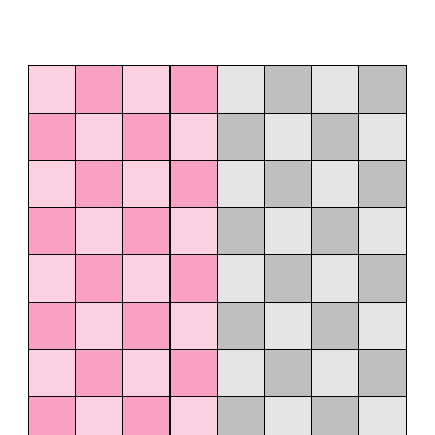
\begin{tikzpicture}[scale=0.6]
			\draw[fill=WildStrawberry, fill opacity=0.4] (0, 0) -- (0, 1) -- (1, 1) -- (1, 0) -- (0, 0);
\draw[fill=WildStrawberry, fill opacity=0.2] (0, 1) -- (0, 2) -- (1, 2) -- (1, 1) -- (0, 1);
\draw[fill=WildStrawberry, fill opacity=0.4] (0, 2) -- (0, 3) -- (1, 3) -- (1, 2) -- (0, 2);
\draw[fill=WildStrawberry, fill opacity=0.2] (0, 3) -- (0, 4) -- (1, 4) -- (1, 3) -- (0, 3);
\draw[fill=WildStrawberry, fill opacity=0.4] (0, 4) -- (0, 5) -- (1, 5) -- (1, 4) -- (0, 4);
\draw[fill=WildStrawberry, fill opacity=0.2] (0, 5) -- (0, 6) -- (1, 6) -- (1, 5) -- (0, 5);
\draw[fill=WildStrawberry, fill opacity=0.4] (0, 6) -- (0, 7) -- (1, 7) -- (1, 6) -- (0, 6);
\draw[fill=WildStrawberry, fill opacity=0.2] (0, 7) -- (0, 8) -- (1, 8) -- (1, 7) -- (0, 7);
\draw[fill=WildStrawberry, fill opacity=0.2] (1, 0) -- (1, 1) -- (2, 1) -- (2, 0) -- (1, 0);
\draw[fill=WildStrawberry, fill opacity=0.4] (1, 1) -- (1, 2) -- (2, 2) -- (2, 1) -- (1, 1);
\draw[fill=WildStrawberry, fill opacity=0.2] (1, 2) -- (1, 3) -- (2, 3) -- (2, 2) -- (1, 2);
\draw[fill=WildStrawberry, fill opacity=0.4] (1, 3) -- (1, 4) -- (2, 4) -- (2, 3) -- (1, 3);
\draw[fill=WildStrawberry, fill opacity=0.2] (1, 4) -- (1, 5) -- (2, 5) -- (2, 4) -- (1, 4);
\draw[fill=WildStrawberry, fill opacity=0.4] (1, 5) -- (1, 6) -- (2, 6) -- (2, 5) -- (1, 5);
\draw[fill=WildStrawberry, fill opacity=0.2] (1, 6) -- (1, 7) -- (2, 7) -- (2, 6) -- (1, 6);
\draw[fill=WildStrawberry, fill opacity=0.4] (1, 7) -- (1, 8) -- (2, 8) -- (2, 7) -- (1, 7);
\draw[fill=WildStrawberry, fill opacity=0.4] (2, 0) -- (2, 1) -- (3, 1) -- (3, 0) -- (2, 0);
\draw[fill=WildStrawberry, fill opacity=0.2] (2, 1) -- (2, 2) -- (3, 2) -- (3, 1) -- (2, 1);
\draw[fill=WildStrawberry, fill opacity=0.4] (2, 2) -- (2, 3) -- (3, 3) -- (3, 2) -- (2, 2);
\draw[fill=WildStrawberry, fill opacity=0.2] (2, 3) -- (2, 4) -- (3, 4) -- (3, 3) -- (2, 3);
\draw[fill=WildStrawberry, fill opacity=0.4] (2, 4) -- (2, 5) -- (3, 5) -- (3, 4) -- (2, 4);
\draw[fill=WildStrawberry, fill opacity=0.2] (2, 5) -- (2, 6) -- (3, 6) -- (3, 5) -- (2, 5);
\draw[fill=WildStrawberry, fill opacity=0.4] (2, 6) -- (2, 7) -- (3, 7) -- (3, 6) -- (2, 6);
\draw[fill=WildStrawberry, fill opacity=0.2] (2, 7) -- (2, 8) -- (3, 8) -- (3, 7) -- (2, 7);
\draw[fill=WildStrawberry, fill opacity=0.2] (3, 0) -- (3, 1) -- (4, 1) -- (4, 0) -- (3, 0);
\draw[fill=WildStrawberry, fill opacity=0.4] (3, 1) -- (3, 2) -- (4, 2) -- (4, 1) -- (3, 1);
\draw[fill=WildStrawberry, fill opacity=0.2] (3, 2) -- (3, 3) -- (4, 3) -- (4, 2) -- (3, 2);
\draw[fill=WildStrawberry, fill opacity=0.4] (3, 3) -- (3, 4) -- (4, 4) -- (4, 3) -- (3, 3);
\draw[fill=WildStrawberry, fill opacity=0.2] (3, 4) -- (3, 5) -- (4, 5) -- (4, 4) -- (3, 4);
\draw[fill=WildStrawberry, fill opacity=0.4] (3, 5) -- (3, 6) -- (4, 6) -- (4, 5) -- (3, 5);
\draw[fill=WildStrawberry, fill opacity=0.2] (3, 6) -- (3, 7) -- (4, 7) -- (4, 6) -- (3, 6);
\draw[fill=WildStrawberry, fill opacity=0.4] (3, 7) -- (3, 8) -- (4, 8) -- (4, 7) -- (3, 7);
\draw[fill=black, fill opacity=0.25] (4, 0) -- (4, 1) -- (5, 1) -- (5, 0) -- (4, 0);
\draw[fill=black, fill opacity=0.1] (4, 1) -- (4, 2) -- (5, 2) -- (5, 1) -- (4, 1);
\draw[fill=black, fill opacity=0.25] (4, 2) -- (4, 3) -- (5, 3) -- (5, 2) -- (4, 2);
\draw[fill=black, fill opacity=0.1] (4, 3) -- (4, 4) -- (5, 4) -- (5, 3) -- (4, 3);
\draw[fill=black, fill opacity=0.25] (4, 4) -- (4, 5) -- (5, 5) -- (5, 4) -- (4, 4);
\draw[fill=black, fill opacity=0.1] (4, 5) -- (4, 6) -- (5, 6) -- (5, 5) -- (4, 5);
\draw[fill=black, fill opacity=0.25] (4, 6) -- (4, 7) -- (5, 7) -- (5, 6) -- (4, 6);
\draw[fill=black, fill opacity=0.1] (4, 7) -- (4, 8) -- (5, 8) -- (5, 7) -- (4, 7);
\draw[fill=black, fill opacity=0.1] (5, 0) -- (5, 1) -- (6, 1) -- (6, 0) -- (5, 0);
\draw[fill=black, fill opacity=0.25] (5, 1) -- (5, 2) -- (6, 2) -- (6, 1) -- (5, 1);
\draw[fill=black, fill opacity=0.1] (5, 2) -- (5, 3) -- (6, 3) -- (6, 2) -- (5, 2);
\draw[fill=black, fill opacity=0.25] (5, 3) -- (5, 4) -- (6, 4) -- (6, 3) -- (5, 3);
\draw[fill=black, fill opacity=0.1] (5, 4) -- (5, 5) -- (6, 5) -- (6, 4) -- (5, 4);
\draw[fill=black, fill opacity=0.25] (5, 5) -- (5, 6) -- (6, 6) -- (6, 5) -- (5, 5);
\draw[fill=black, fill opacity=0.1] (5, 6) -- (5, 7) -- (6, 7) -- (6, 6) -- (5, 6);
\draw[fill=black, fill opacity=0.25] (5, 7) -- (5, 8) -- (6, 8) -- (6, 7) -- (5, 7);
\draw[fill=black, fill opacity=0.25] (6, 0) -- (6, 1) -- (7, 1) -- (7, 0) -- (6, 0);
\draw[fill=black, fill opacity=0.1] (6, 1) -- (6, 2) -- (7, 2) -- (7, 1) -- (6, 1);
\draw[fill=black, fill opacity=0.25] (6, 2) -- (6, 3) -- (7, 3) -- (7, 2) -- (6, 2);
\draw[fill=black, fill opacity=0.1] (6, 3) -- (6, 4) -- (7, 4) -- (7, 3) -- (6, 3);
\draw[fill=black, fill opacity=0.25] (6, 4) -- (6, 5) -- (7, 5) -- (7, 4) -- (6, 4);
\draw[fill=black, fill opacity=0.1] (6, 5) -- (6, 6) -- (7, 6) -- (7, 5) -- (6, 5);
\draw[fill=black, fill opacity=0.25] (6, 6) -- (6, 7) -- (7, 7) -- (7, 6) -- (6, 6);
\draw[fill=black, fill opacity=0.1] (6, 7) -- (6, 8) -- (7, 8) -- (7, 7) -- (6, 7);
\draw[fill=black, fill opacity=0.1] (7, 0) -- (7, 1) -- (8, 1) -- (8, 0) -- (7, 0);
\draw[fill=black, fill opacity=0.25] (7, 1) -- (7, 2) -- (8, 2) -- (8, 1) -- (7, 1);
\draw[fill=black, fill opacity=0.1] (7, 2) -- (7, 3) -- (8, 3) -- (8, 2) -- (7, 2);
\draw[fill=black, fill opacity=0.25] (7, 3) -- (7, 4) -- (8, 4) -- (8, 3) -- (7, 3);
\draw[fill=black, fill opacity=0.1] (7, 4) -- (7, 5) -- (8, 5) -- (8, 4) -- (7, 4);
\draw[fill=black, fill opacity=0.25] (7, 5) -- (7, 6) -- (8, 6) -- (8, 5) -- (7, 5);
\draw[fill=black, fill opacity=0.1] (7, 6) -- (7, 7) -- (8, 7) -- (8, 6) -- (7, 6);
\draw[fill=black, fill opacity=0.25] (7, 7) -- (7, 8) -- (8, 8) -- (8, 7) -- (7, 7);
		\end{tikzpicture}\hspace{5mm}
		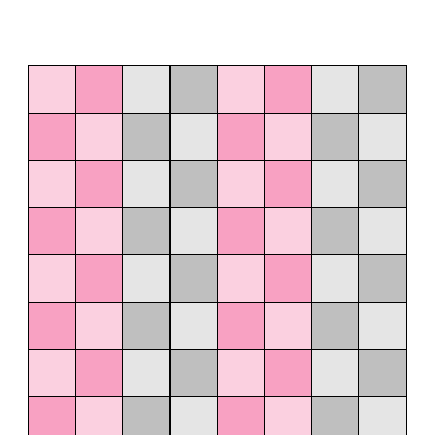
\begin{tikzpicture}[scale=0.6]
			\draw[fill=WildStrawberry, fill opacity=0.4] (0, 0) -- (0, 1) -- (1, 1) -- (1, 0) -- (0, 0);
\draw[fill=WildStrawberry, fill opacity=0.2] (0, 1) -- (0, 2) -- (1, 2) -- (1, 1) -- (0, 1);
\draw[fill=WildStrawberry, fill opacity=0.4] (0, 2) -- (0, 3) -- (1, 3) -- (1, 2) -- (0, 2);
\draw[fill=WildStrawberry, fill opacity=0.2] (0, 3) -- (0, 4) -- (1, 4) -- (1, 3) -- (0, 3);
\draw[fill=WildStrawberry, fill opacity=0.4] (0, 4) -- (0, 5) -- (1, 5) -- (1, 4) -- (0, 4);
\draw[fill=WildStrawberry, fill opacity=0.2] (0, 5) -- (0, 6) -- (1, 6) -- (1, 5) -- (0, 5);
\draw[fill=WildStrawberry, fill opacity=0.4] (0, 6) -- (0, 7) -- (1, 7) -- (1, 6) -- (0, 6);
\draw[fill=WildStrawberry, fill opacity=0.2] (0, 7) -- (0, 8) -- (1, 8) -- (1, 7) -- (0, 7);
\draw[fill=WildStrawberry, fill opacity=0.2] (1, 0) -- (1, 1) -- (2, 1) -- (2, 0) -- (1, 0);
\draw[fill=WildStrawberry, fill opacity=0.4] (1, 1) -- (1, 2) -- (2, 2) -- (2, 1) -- (1, 1);
\draw[fill=WildStrawberry, fill opacity=0.2] (1, 2) -- (1, 3) -- (2, 3) -- (2, 2) -- (1, 2);
\draw[fill=WildStrawberry, fill opacity=0.4] (1, 3) -- (1, 4) -- (2, 4) -- (2, 3) -- (1, 3);
\draw[fill=WildStrawberry, fill opacity=0.2] (1, 4) -- (1, 5) -- (2, 5) -- (2, 4) -- (1, 4);
\draw[fill=WildStrawberry, fill opacity=0.4] (1, 5) -- (1, 6) -- (2, 6) -- (2, 5) -- (1, 5);
\draw[fill=WildStrawberry, fill opacity=0.2] (1, 6) -- (1, 7) -- (2, 7) -- (2, 6) -- (1, 6);
\draw[fill=WildStrawberry, fill opacity=0.4] (1, 7) -- (1, 8) -- (2, 8) -- (2, 7) -- (1, 7);
\draw[fill=black, fill opacity=0.25] (2, 0) -- (2, 1) -- (3, 1) -- (3, 0) -- (2, 0);
\draw[fill=black, fill opacity=0.1] (2, 1) -- (2, 2) -- (3, 2) -- (3, 1) -- (2, 1);
\draw[fill=black, fill opacity=0.25] (2, 2) -- (2, 3) -- (3, 3) -- (3, 2) -- (2, 2);
\draw[fill=black, fill opacity=0.1] (2, 3) -- (2, 4) -- (3, 4) -- (3, 3) -- (2, 3);
\draw[fill=black, fill opacity=0.25] (2, 4) -- (2, 5) -- (3, 5) -- (3, 4) -- (2, 4);
\draw[fill=black, fill opacity=0.1] (2, 5) -- (2, 6) -- (3, 6) -- (3, 5) -- (2, 5);
\draw[fill=black, fill opacity=0.25] (2, 6) -- (2, 7) -- (3, 7) -- (3, 6) -- (2, 6);
\draw[fill=black, fill opacity=0.1] (2, 7) -- (2, 8) -- (3, 8) -- (3, 7) -- (2, 7);
\draw[fill=black, fill opacity=0.1] (3, 0) -- (3, 1) -- (4, 1) -- (4, 0) -- (3, 0);
\draw[fill=black, fill opacity=0.25] (3, 1) -- (3, 2) -- (4, 2) -- (4, 1) -- (3, 1);
\draw[fill=black, fill opacity=0.1] (3, 2) -- (3, 3) -- (4, 3) -- (4, 2) -- (3, 2);
\draw[fill=black, fill opacity=0.25] (3, 3) -- (3, 4) -- (4, 4) -- (4, 3) -- (3, 3);
\draw[fill=black, fill opacity=0.1] (3, 4) -- (3, 5) -- (4, 5) -- (4, 4) -- (3, 4);
\draw[fill=black, fill opacity=0.25] (3, 5) -- (3, 6) -- (4, 6) -- (4, 5) -- (3, 5);
\draw[fill=black, fill opacity=0.1] (3, 6) -- (3, 7) -- (4, 7) -- (4, 6) -- (3, 6);
\draw[fill=black, fill opacity=0.25] (3, 7) -- (3, 8) -- (4, 8) -- (4, 7) -- (3, 7);
\draw[fill=WildStrawberry, fill opacity=0.4] (4, 0) -- (4, 1) -- (5, 1) -- (5, 0) -- (4, 0);
\draw[fill=WildStrawberry, fill opacity=0.2] (4, 1) -- (4, 2) -- (5, 2) -- (5, 1) -- (4, 1);
\draw[fill=WildStrawberry, fill opacity=0.4] (4, 2) -- (4, 3) -- (5, 3) -- (5, 2) -- (4, 2);
\draw[fill=WildStrawberry, fill opacity=0.2] (4, 3) -- (4, 4) -- (5, 4) -- (5, 3) -- (4, 3);
\draw[fill=WildStrawberry, fill opacity=0.4] (4, 4) -- (4, 5) -- (5, 5) -- (5, 4) -- (4, 4);
\draw[fill=WildStrawberry, fill opacity=0.2] (4, 5) -- (4, 6) -- (5, 6) -- (5, 5) -- (4, 5);
\draw[fill=WildStrawberry, fill opacity=0.4] (4, 6) -- (4, 7) -- (5, 7) -- (5, 6) -- (4, 6);
\draw[fill=WildStrawberry, fill opacity=0.2] (4, 7) -- (4, 8) -- (5, 8) -- (5, 7) -- (4, 7);
\draw[fill=WildStrawberry, fill opacity=0.2] (5, 0) -- (5, 1) -- (6, 1) -- (6, 0) -- (5, 0);
\draw[fill=WildStrawberry, fill opacity=0.4] (5, 1) -- (5, 2) -- (6, 2) -- (6, 1) -- (5, 1);
\draw[fill=WildStrawberry, fill opacity=0.2] (5, 2) -- (5, 3) -- (6, 3) -- (6, 2) -- (5, 2);
\draw[fill=WildStrawberry, fill opacity=0.4] (5, 3) -- (5, 4) -- (6, 4) -- (6, 3) -- (5, 3);
\draw[fill=WildStrawberry, fill opacity=0.2] (5, 4) -- (5, 5) -- (6, 5) -- (6, 4) -- (5, 4);
\draw[fill=WildStrawberry, fill opacity=0.4] (5, 5) -- (5, 6) -- (6, 6) -- (6, 5) -- (5, 5);
\draw[fill=WildStrawberry, fill opacity=0.2] (5, 6) -- (5, 7) -- (6, 7) -- (6, 6) -- (5, 6);
\draw[fill=WildStrawberry, fill opacity=0.4] (5, 7) -- (5, 8) -- (6, 8) -- (6, 7) -- (5, 7);
\draw[fill=black, fill opacity=0.25] (6, 0) -- (6, 1) -- (7, 1) -- (7, 0) -- (6, 0);
\draw[fill=black, fill opacity=0.1] (6, 1) -- (6, 2) -- (7, 2) -- (7, 1) -- (6, 1);
\draw[fill=black, fill opacity=0.25] (6, 2) -- (6, 3) -- (7, 3) -- (7, 2) -- (6, 2);
\draw[fill=black, fill opacity=0.1] (6, 3) -- (6, 4) -- (7, 4) -- (7, 3) -- (6, 3);
\draw[fill=black, fill opacity=0.25] (6, 4) -- (6, 5) -- (7, 5) -- (7, 4) -- (6, 4);
\draw[fill=black, fill opacity=0.1] (6, 5) -- (6, 6) -- (7, 6) -- (7, 5) -- (6, 5);
\draw[fill=black, fill opacity=0.25] (6, 6) -- (6, 7) -- (7, 7) -- (7, 6) -- (6, 6);
\draw[fill=black, fill opacity=0.1] (6, 7) -- (6, 8) -- (7, 8) -- (7, 7) -- (6, 7);
\draw[fill=black, fill opacity=0.1] (7, 0) -- (7, 1) -- (8, 1) -- (8, 0) -- (7, 0);
\draw[fill=black, fill opacity=0.25] (7, 1) -- (7, 2) -- (8, 2) -- (8, 1) -- (7, 1);
\draw[fill=black, fill opacity=0.1] (7, 2) -- (7, 3) -- (8, 3) -- (8, 2) -- (7, 2);
\draw[fill=black, fill opacity=0.25] (7, 3) -- (7, 4) -- (8, 4) -- (8, 3) -- (7, 3);
\draw[fill=black, fill opacity=0.1] (7, 4) -- (7, 5) -- (8, 5) -- (8, 4) -- (7, 4);
\draw[fill=black, fill opacity=0.25] (7, 5) -- (7, 6) -- (8, 6) -- (8, 5) -- (7, 5);
\draw[fill=black, fill opacity=0.1] (7, 6) -- (7, 7) -- (8, 7) -- (8, 6) -- (7, 6);
\draw[fill=black, fill opacity=0.25] (7, 7) -- (7, 8) -- (8, 8) -- (8, 7) -- (7, 7);
		\end{tikzpicture}\hspace{5mm}
		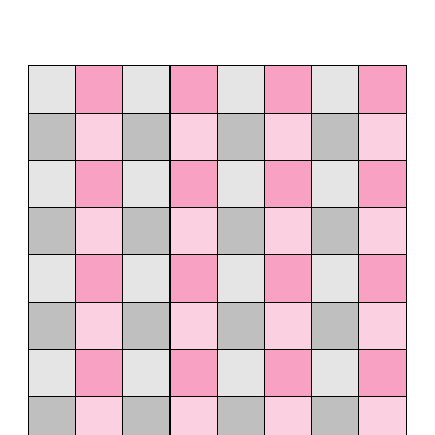
\begin{tikzpicture}[scale=0.6]
			\draw[fill=black, fill opacity=0.25] (0, 0) -- (0, 1) -- (1, 1) -- (1, 0) -- (0, 0);
\draw[fill=WildStrawberry, fill opacity=0.2] (1, 0) -- (1, 1) -- (2, 1) -- (2, 0) -- (1, 0);
\draw[fill=black, fill opacity=0.25] (2, 0) -- (2, 1) -- (3, 1) -- (3, 0) -- (2, 0);
\draw[fill=WildStrawberry, fill opacity=0.2] (3, 0) -- (3, 1) -- (4, 1) -- (4, 0) -- (3, 0);
\draw[fill=black, fill opacity=0.25] (4, 0) -- (4, 1) -- (5, 1) -- (5, 0) -- (4, 0);
\draw[fill=WildStrawberry, fill opacity=0.2] (5, 0) -- (5, 1) -- (6, 1) -- (6, 0) -- (5, 0);
\draw[fill=black, fill opacity=0.25] (6, 0) -- (6, 1) -- (7, 1) -- (7, 0) -- (6, 0);
\draw[fill=WildStrawberry, fill opacity=0.2] (7, 0) -- (7, 1) -- (8, 1) -- (8, 0) -- (7, 0);
\draw[fill=black, fill opacity=0.1] (0, 1) -- (0, 2) -- (1, 2) -- (1, 1) -- (0, 1);
\draw[fill=WildStrawberry, fill opacity=0.4] (1, 1) -- (1, 2) -- (2, 2) -- (2, 1) -- (1, 1);
\draw[fill=black, fill opacity=0.1] (2, 1) -- (2, 2) -- (3, 2) -- (3, 1) -- (2, 1);
\draw[fill=WildStrawberry, fill opacity=0.4] (3, 1) -- (3, 2) -- (4, 2) -- (4, 1) -- (3, 1);
\draw[fill=black, fill opacity=0.1] (4, 1) -- (4, 2) -- (5, 2) -- (5, 1) -- (4, 1);
\draw[fill=WildStrawberry, fill opacity=0.4] (5, 1) -- (5, 2) -- (6, 2) -- (6, 1) -- (5, 1);
\draw[fill=black, fill opacity=0.1] (6, 1) -- (6, 2) -- (7, 2) -- (7, 1) -- (6, 1);
\draw[fill=WildStrawberry, fill opacity=0.4] (7, 1) -- (7, 2) -- (8, 2) -- (8, 1) -- (7, 1);
\draw[fill=black, fill opacity=0.25] (0, 2) -- (0, 3) -- (1, 3) -- (1, 2) -- (0, 2);
\draw[fill=WildStrawberry, fill opacity=0.2] (1, 2) -- (1, 3) -- (2, 3) -- (2, 2) -- (1, 2);
\draw[fill=black, fill opacity=0.25] (2, 2) -- (2, 3) -- (3, 3) -- (3, 2) -- (2, 2);
\draw[fill=WildStrawberry, fill opacity=0.2] (3, 2) -- (3, 3) -- (4, 3) -- (4, 2) -- (3, 2);
\draw[fill=black, fill opacity=0.25] (4, 2) -- (4, 3) -- (5, 3) -- (5, 2) -- (4, 2);
\draw[fill=WildStrawberry, fill opacity=0.2] (5, 2) -- (5, 3) -- (6, 3) -- (6, 2) -- (5, 2);
\draw[fill=black, fill opacity=0.25] (6, 2) -- (6, 3) -- (7, 3) -- (7, 2) -- (6, 2);
\draw[fill=WildStrawberry, fill opacity=0.2] (7, 2) -- (7, 3) -- (8, 3) -- (8, 2) -- (7, 2);
\draw[fill=black, fill opacity=0.1] (0, 3) -- (0, 4) -- (1, 4) -- (1, 3) -- (0, 3);
\draw[fill=WildStrawberry, fill opacity=0.4] (1, 3) -- (1, 4) -- (2, 4) -- (2, 3) -- (1, 3);
\draw[fill=black, fill opacity=0.1] (2, 3) -- (2, 4) -- (3, 4) -- (3, 3) -- (2, 3);
\draw[fill=WildStrawberry, fill opacity=0.4] (3, 3) -- (3, 4) -- (4, 4) -- (4, 3) -- (3, 3);
\draw[fill=black, fill opacity=0.1] (4, 3) -- (4, 4) -- (5, 4) -- (5, 3) -- (4, 3);
\draw[fill=WildStrawberry, fill opacity=0.4] (5, 3) -- (5, 4) -- (6, 4) -- (6, 3) -- (5, 3);
\draw[fill=black, fill opacity=0.1] (6, 3) -- (6, 4) -- (7, 4) -- (7, 3) -- (6, 3);
\draw[fill=WildStrawberry, fill opacity=0.4] (7, 3) -- (7, 4) -- (8, 4) -- (8, 3) -- (7, 3);
\draw[fill=black, fill opacity=0.25] (0, 4) -- (0, 5) -- (1, 5) -- (1, 4) -- (0, 4);
\draw[fill=WildStrawberry, fill opacity=0.2] (1, 4) -- (1, 5) -- (2, 5) -- (2, 4) -- (1, 4);
\draw[fill=black, fill opacity=0.25] (2, 4) -- (2, 5) -- (3, 5) -- (3, 4) -- (2, 4);
\draw[fill=WildStrawberry, fill opacity=0.2] (3, 4) -- (3, 5) -- (4, 5) -- (4, 4) -- (3, 4);
\draw[fill=black, fill opacity=0.25] (4, 4) -- (4, 5) -- (5, 5) -- (5, 4) -- (4, 4);
\draw[fill=WildStrawberry, fill opacity=0.2] (5, 4) -- (5, 5) -- (6, 5) -- (6, 4) -- (5, 4);
\draw[fill=black, fill opacity=0.25] (6, 4) -- (6, 5) -- (7, 5) -- (7, 4) -- (6, 4);
\draw[fill=WildStrawberry, fill opacity=0.2] (7, 4) -- (7, 5) -- (8, 5) -- (8, 4) -- (7, 4);
\draw[fill=black, fill opacity=0.1] (0, 5) -- (0, 6) -- (1, 6) -- (1, 5) -- (0, 5);
\draw[fill=WildStrawberry, fill opacity=0.4] (1, 5) -- (1, 6) -- (2, 6) -- (2, 5) -- (1, 5);
\draw[fill=black, fill opacity=0.1] (2, 5) -- (2, 6) -- (3, 6) -- (3, 5) -- (2, 5);
\draw[fill=WildStrawberry, fill opacity=0.4] (3, 5) -- (3, 6) -- (4, 6) -- (4, 5) -- (3, 5);
\draw[fill=black, fill opacity=0.1] (4, 5) -- (4, 6) -- (5, 6) -- (5, 5) -- (4, 5);
\draw[fill=WildStrawberry, fill opacity=0.4] (5, 5) -- (5, 6) -- (6, 6) -- (6, 5) -- (5, 5);
\draw[fill=black, fill opacity=0.1] (6, 5) -- (6, 6) -- (7, 6) -- (7, 5) -- (6, 5);
\draw[fill=WildStrawberry, fill opacity=0.4] (7, 5) -- (7, 6) -- (8, 6) -- (8, 5) -- (7, 5);
\draw[fill=black, fill opacity=0.25] (0, 6) -- (0, 7) -- (1, 7) -- (1, 6) -- (0, 6);
\draw[fill=WildStrawberry, fill opacity=0.2] (1, 6) -- (1, 7) -- (2, 7) -- (2, 6) -- (1, 6);
\draw[fill=black, fill opacity=0.25] (2, 6) -- (2, 7) -- (3, 7) -- (3, 6) -- (2, 6);
\draw[fill=WildStrawberry, fill opacity=0.2] (3, 6) -- (3, 7) -- (4, 7) -- (4, 6) -- (3, 6);
\draw[fill=black, fill opacity=0.25] (4, 6) -- (4, 7) -- (5, 7) -- (5, 6) -- (4, 6);
\draw[fill=WildStrawberry, fill opacity=0.2] (5, 6) -- (5, 7) -- (6, 7) -- (6, 6) -- (5, 6);
\draw[fill=black, fill opacity=0.25] (6, 6) -- (6, 7) -- (7, 7) -- (7, 6) -- (6, 6);
\draw[fill=WildStrawberry, fill opacity=0.2] (7, 6) -- (7, 7) -- (8, 7) -- (8, 6) -- (7, 6);
\draw[fill=black, fill opacity=0.1] (0, 7) -- (0, 8) -- (1, 8) -- (1, 7) -- (0, 7);
\draw[fill=WildStrawberry, fill opacity=0.4] (1, 7) -- (1, 8) -- (2, 8) -- (2, 7) -- (1, 7);
\draw[fill=black, fill opacity=0.1] (2, 7) -- (2, 8) -- (3, 8) -- (3, 7) -- (2, 7);
\draw[fill=WildStrawberry, fill opacity=0.4] (3, 7) -- (3, 8) -- (4, 8) -- (4, 7) -- (3, 7);
\draw[fill=black, fill opacity=0.1] (4, 7) -- (4, 8) -- (5, 8) -- (5, 7) -- (4, 7);
\draw[fill=WildStrawberry, fill opacity=0.4] (5, 7) -- (5, 8) -- (6, 8) -- (6, 7) -- (5, 7);
\draw[fill=black, fill opacity=0.1] (6, 7) -- (6, 8) -- (7, 8) -- (7, 7) -- (6, 7);
\draw[fill=WildStrawberry, fill opacity=0.4] (7, 7) -- (7, 8) -- (8, 8) -- (8, 7) -- (7, 7);
		\end{tikzpicture}\vspace{6mm}
		\\
		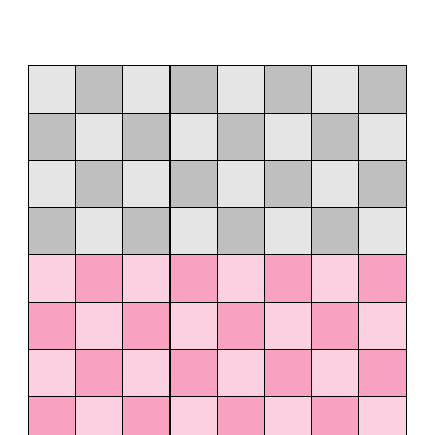
\begin{tikzpicture}[scale=0.6]
			\draw[fill=WildStrawberry, fill opacity=0.4] (0, 0) -- (0, 1) -- (1, 1) -- (1, 0) -- (0, 0);
\draw[fill=WildStrawberry, fill opacity=0.2] (1, 0) -- (1, 1) -- (2, 1) -- (2, 0) -- (1, 0);
\draw[fill=WildStrawberry, fill opacity=0.4] (2, 0) -- (2, 1) -- (3, 1) -- (3, 0) -- (2, 0);
\draw[fill=WildStrawberry, fill opacity=0.2] (3, 0) -- (3, 1) -- (4, 1) -- (4, 0) -- (3, 0);
\draw[fill=WildStrawberry, fill opacity=0.4] (4, 0) -- (4, 1) -- (5, 1) -- (5, 0) -- (4, 0);
\draw[fill=WildStrawberry, fill opacity=0.2] (5, 0) -- (5, 1) -- (6, 1) -- (6, 0) -- (5, 0);
\draw[fill=WildStrawberry, fill opacity=0.4] (6, 0) -- (6, 1) -- (7, 1) -- (7, 0) -- (6, 0);
\draw[fill=WildStrawberry, fill opacity=0.2] (7, 0) -- (7, 1) -- (8, 1) -- (8, 0) -- (7, 0);
\draw[fill=WildStrawberry, fill opacity=0.2] (0, 1) -- (0, 2) -- (1, 2) -- (1, 1) -- (0, 1);
\draw[fill=WildStrawberry, fill opacity=0.4] (1, 1) -- (1, 2) -- (2, 2) -- (2, 1) -- (1, 1);
\draw[fill=WildStrawberry, fill opacity=0.2] (2, 1) -- (2, 2) -- (3, 2) -- (3, 1) -- (2, 1);
\draw[fill=WildStrawberry, fill opacity=0.4] (3, 1) -- (3, 2) -- (4, 2) -- (4, 1) -- (3, 1);
\draw[fill=WildStrawberry, fill opacity=0.2] (4, 1) -- (4, 2) -- (5, 2) -- (5, 1) -- (4, 1);
\draw[fill=WildStrawberry, fill opacity=0.4] (5, 1) -- (5, 2) -- (6, 2) -- (6, 1) -- (5, 1);
\draw[fill=WildStrawberry, fill opacity=0.2] (6, 1) -- (6, 2) -- (7, 2) -- (7, 1) -- (6, 1);
\draw[fill=WildStrawberry, fill opacity=0.4] (7, 1) -- (7, 2) -- (8, 2) -- (8, 1) -- (7, 1);
\draw[fill=WildStrawberry, fill opacity=0.4] (0, 2) -- (0, 3) -- (1, 3) -- (1, 2) -- (0, 2);
\draw[fill=WildStrawberry, fill opacity=0.2] (1, 2) -- (1, 3) -- (2, 3) -- (2, 2) -- (1, 2);
\draw[fill=WildStrawberry, fill opacity=0.4] (2, 2) -- (2, 3) -- (3, 3) -- (3, 2) -- (2, 2);
\draw[fill=WildStrawberry, fill opacity=0.2] (3, 2) -- (3, 3) -- (4, 3) -- (4, 2) -- (3, 2);
\draw[fill=WildStrawberry, fill opacity=0.4] (4, 2) -- (4, 3) -- (5, 3) -- (5, 2) -- (4, 2);
\draw[fill=WildStrawberry, fill opacity=0.2] (5, 2) -- (5, 3) -- (6, 3) -- (6, 2) -- (5, 2);
\draw[fill=WildStrawberry, fill opacity=0.4] (6, 2) -- (6, 3) -- (7, 3) -- (7, 2) -- (6, 2);
\draw[fill=WildStrawberry, fill opacity=0.2] (7, 2) -- (7, 3) -- (8, 3) -- (8, 2) -- (7, 2);
\draw[fill=WildStrawberry, fill opacity=0.2] (0, 3) -- (0, 4) -- (1, 4) -- (1, 3) -- (0, 3);
\draw[fill=WildStrawberry, fill opacity=0.4] (1, 3) -- (1, 4) -- (2, 4) -- (2, 3) -- (1, 3);
\draw[fill=WildStrawberry, fill opacity=0.2] (2, 3) -- (2, 4) -- (3, 4) -- (3, 3) -- (2, 3);
\draw[fill=WildStrawberry, fill opacity=0.4] (3, 3) -- (3, 4) -- (4, 4) -- (4, 3) -- (3, 3);
\draw[fill=WildStrawberry, fill opacity=0.2] (4, 3) -- (4, 4) -- (5, 4) -- (5, 3) -- (4, 3);
\draw[fill=WildStrawberry, fill opacity=0.4] (5, 3) -- (5, 4) -- (6, 4) -- (6, 3) -- (5, 3);
\draw[fill=WildStrawberry, fill opacity=0.2] (6, 3) -- (6, 4) -- (7, 4) -- (7, 3) -- (6, 3);
\draw[fill=WildStrawberry, fill opacity=0.4] (7, 3) -- (7, 4) -- (8, 4) -- (8, 3) -- (7, 3);
\draw[fill=black, fill opacity=0.25] (0, 4) -- (0, 5) -- (1, 5) -- (1, 4) -- (0, 4);
\draw[fill=black, fill opacity=0.1] (1, 4) -- (1, 5) -- (2, 5) -- (2, 4) -- (1, 4);
\draw[fill=black, fill opacity=0.25] (2, 4) -- (2, 5) -- (3, 5) -- (3, 4) -- (2, 4);
\draw[fill=black, fill opacity=0.1] (3, 4) -- (3, 5) -- (4, 5) -- (4, 4) -- (3, 4);
\draw[fill=black, fill opacity=0.25] (4, 4) -- (4, 5) -- (5, 5) -- (5, 4) -- (4, 4);
\draw[fill=black, fill opacity=0.1] (5, 4) -- (5, 5) -- (6, 5) -- (6, 4) -- (5, 4);
\draw[fill=black, fill opacity=0.25] (6, 4) -- (6, 5) -- (7, 5) -- (7, 4) -- (6, 4);
\draw[fill=black, fill opacity=0.1] (7, 4) -- (7, 5) -- (8, 5) -- (8, 4) -- (7, 4);
\draw[fill=black, fill opacity=0.1] (0, 5) -- (0, 6) -- (1, 6) -- (1, 5) -- (0, 5);
\draw[fill=black, fill opacity=0.25] (1, 5) -- (1, 6) -- (2, 6) -- (2, 5) -- (1, 5);
\draw[fill=black, fill opacity=0.1] (2, 5) -- (2, 6) -- (3, 6) -- (3, 5) -- (2, 5);
\draw[fill=black, fill opacity=0.25] (3, 5) -- (3, 6) -- (4, 6) -- (4, 5) -- (3, 5);
\draw[fill=black, fill opacity=0.1] (4, 5) -- (4, 6) -- (5, 6) -- (5, 5) -- (4, 5);
\draw[fill=black, fill opacity=0.25] (5, 5) -- (5, 6) -- (6, 6) -- (6, 5) -- (5, 5);
\draw[fill=black, fill opacity=0.1] (6, 5) -- (6, 6) -- (7, 6) -- (7, 5) -- (6, 5);
\draw[fill=black, fill opacity=0.25] (7, 5) -- (7, 6) -- (8, 6) -- (8, 5) -- (7, 5);
\draw[fill=black, fill opacity=0.25] (0, 6) -- (0, 7) -- (1, 7) -- (1, 6) -- (0, 6);
\draw[fill=black, fill opacity=0.1] (1, 6) -- (1, 7) -- (2, 7) -- (2, 6) -- (1, 6);
\draw[fill=black, fill opacity=0.25] (2, 6) -- (2, 7) -- (3, 7) -- (3, 6) -- (2, 6);
\draw[fill=black, fill opacity=0.1] (3, 6) -- (3, 7) -- (4, 7) -- (4, 6) -- (3, 6);
\draw[fill=black, fill opacity=0.25] (4, 6) -- (4, 7) -- (5, 7) -- (5, 6) -- (4, 6);
\draw[fill=black, fill opacity=0.1] (5, 6) -- (5, 7) -- (6, 7) -- (6, 6) -- (5, 6);
\draw[fill=black, fill opacity=0.25] (6, 6) -- (6, 7) -- (7, 7) -- (7, 6) -- (6, 6);
\draw[fill=black, fill opacity=0.1] (7, 6) -- (7, 7) -- (8, 7) -- (8, 6) -- (7, 6);
\draw[fill=black, fill opacity=0.1] (0, 7) -- (0, 8) -- (1, 8) -- (1, 7) -- (0, 7);
\draw[fill=black, fill opacity=0.25] (1, 7) -- (1, 8) -- (2, 8) -- (2, 7) -- (1, 7);
\draw[fill=black, fill opacity=0.1] (2, 7) -- (2, 8) -- (3, 8) -- (3, 7) -- (2, 7);
\draw[fill=black, fill opacity=0.25] (3, 7) -- (3, 8) -- (4, 8) -- (4, 7) -- (3, 7);
\draw[fill=black, fill opacity=0.1] (4, 7) -- (4, 8) -- (5, 8) -- (5, 7) -- (4, 7);
\draw[fill=black, fill opacity=0.25] (5, 7) -- (5, 8) -- (6, 8) -- (6, 7) -- (5, 7);
\draw[fill=black, fill opacity=0.1] (6, 7) -- (6, 8) -- (7, 8) -- (7, 7) -- (6, 7);
\draw[fill=black, fill opacity=0.25] (7, 7) -- (7, 8) -- (8, 8) -- (8, 7) -- (7, 7);
		\end{tikzpicture}\hspace{5mm}
		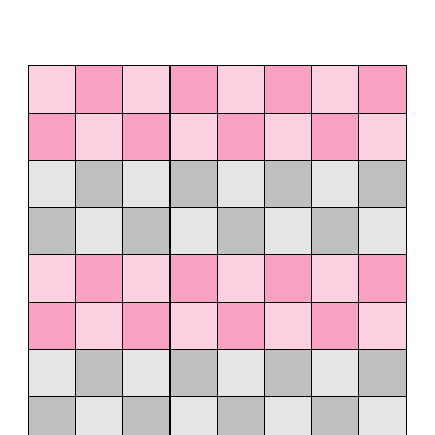
\begin{tikzpicture}[scale=0.6]
			\draw[fill=black, fill opacity=0.25] (0, 0) -- (0, 1) -- (1, 1) -- (1, 0) -- (0, 0);
\draw[fill=black, fill opacity=0.1] (0, 1) -- (0, 2) -- (1, 2) -- (1, 1) -- (0, 1);
\draw[fill=WildStrawberry, fill opacity=0.4] (0, 2) -- (0, 3) -- (1, 3) -- (1, 2) -- (0, 2);
\draw[fill=WildStrawberry, fill opacity=0.2] (0, 3) -- (0, 4) -- (1, 4) -- (1, 3) -- (0, 3);
\draw[fill=black, fill opacity=0.25] (0, 4) -- (0, 5) -- (1, 5) -- (1, 4) -- (0, 4);
\draw[fill=black, fill opacity=0.1] (0, 5) -- (0, 6) -- (1, 6) -- (1, 5) -- (0, 5);
\draw[fill=WildStrawberry, fill opacity=0.4] (0, 6) -- (0, 7) -- (1, 7) -- (1, 6) -- (0, 6);
\draw[fill=WildStrawberry, fill opacity=0.2] (0, 7) -- (0, 8) -- (1, 8) -- (1, 7) -- (0, 7);
\draw[fill=black, fill opacity=0.1] (1, 0) -- (1, 1) -- (2, 1) -- (2, 0) -- (1, 0);
\draw[fill=black, fill opacity=0.25] (1, 1) -- (1, 2) -- (2, 2) -- (2, 1) -- (1, 1);
\draw[fill=WildStrawberry, fill opacity=0.2] (1, 2) -- (1, 3) -- (2, 3) -- (2, 2) -- (1, 2);
\draw[fill=WildStrawberry, fill opacity=0.4] (1, 3) -- (1, 4) -- (2, 4) -- (2, 3) -- (1, 3);
\draw[fill=black, fill opacity=0.1] (1, 4) -- (1, 5) -- (2, 5) -- (2, 4) -- (1, 4);
\draw[fill=black, fill opacity=0.25] (1, 5) -- (1, 6) -- (2, 6) -- (2, 5) -- (1, 5);
\draw[fill=WildStrawberry, fill opacity=0.2] (1, 6) -- (1, 7) -- (2, 7) -- (2, 6) -- (1, 6);
\draw[fill=WildStrawberry, fill opacity=0.4] (1, 7) -- (1, 8) -- (2, 8) -- (2, 7) -- (1, 7);
\draw[fill=black, fill opacity=0.25] (2, 0) -- (2, 1) -- (3, 1) -- (3, 0) -- (2, 0);
\draw[fill=black, fill opacity=0.1] (2, 1) -- (2, 2) -- (3, 2) -- (3, 1) -- (2, 1);
\draw[fill=WildStrawberry, fill opacity=0.4] (2, 2) -- (2, 3) -- (3, 3) -- (3, 2) -- (2, 2);
\draw[fill=WildStrawberry, fill opacity=0.2] (2, 3) -- (2, 4) -- (3, 4) -- (3, 3) -- (2, 3);
\draw[fill=black, fill opacity=0.25] (2, 4) -- (2, 5) -- (3, 5) -- (3, 4) -- (2, 4);
\draw[fill=black, fill opacity=0.1] (2, 5) -- (2, 6) -- (3, 6) -- (3, 5) -- (2, 5);
\draw[fill=WildStrawberry, fill opacity=0.4] (2, 6) -- (2, 7) -- (3, 7) -- (3, 6) -- (2, 6);
\draw[fill=WildStrawberry, fill opacity=0.2] (2, 7) -- (2, 8) -- (3, 8) -- (3, 7) -- (2, 7);
\draw[fill=black, fill opacity=0.1] (3, 0) -- (3, 1) -- (4, 1) -- (4, 0) -- (3, 0);
\draw[fill=black, fill opacity=0.25] (3, 1) -- (3, 2) -- (4, 2) -- (4, 1) -- (3, 1);
\draw[fill=WildStrawberry, fill opacity=0.2] (3, 2) -- (3, 3) -- (4, 3) -- (4, 2) -- (3, 2);
\draw[fill=WildStrawberry, fill opacity=0.4] (3, 3) -- (3, 4) -- (4, 4) -- (4, 3) -- (3, 3);
\draw[fill=black, fill opacity=0.1] (3, 4) -- (3, 5) -- (4, 5) -- (4, 4) -- (3, 4);
\draw[fill=black, fill opacity=0.25] (3, 5) -- (3, 6) -- (4, 6) -- (4, 5) -- (3, 5);
\draw[fill=WildStrawberry, fill opacity=0.2] (3, 6) -- (3, 7) -- (4, 7) -- (4, 6) -- (3, 6);
\draw[fill=WildStrawberry, fill opacity=0.4] (3, 7) -- (3, 8) -- (4, 8) -- (4, 7) -- (3, 7);
\draw[fill=black, fill opacity=0.25] (4, 0) -- (4, 1) -- (5, 1) -- (5, 0) -- (4, 0);
\draw[fill=black, fill opacity=0.1] (4, 1) -- (4, 2) -- (5, 2) -- (5, 1) -- (4, 1);
\draw[fill=WildStrawberry, fill opacity=0.4] (4, 2) -- (4, 3) -- (5, 3) -- (5, 2) -- (4, 2);
\draw[fill=WildStrawberry, fill opacity=0.2] (4, 3) -- (4, 4) -- (5, 4) -- (5, 3) -- (4, 3);
\draw[fill=black, fill opacity=0.25] (4, 4) -- (4, 5) -- (5, 5) -- (5, 4) -- (4, 4);
\draw[fill=black, fill opacity=0.1] (4, 5) -- (4, 6) -- (5, 6) -- (5, 5) -- (4, 5);
\draw[fill=WildStrawberry, fill opacity=0.4] (4, 6) -- (4, 7) -- (5, 7) -- (5, 6) -- (4, 6);
\draw[fill=WildStrawberry, fill opacity=0.2] (4, 7) -- (4, 8) -- (5, 8) -- (5, 7) -- (4, 7);
\draw[fill=black, fill opacity=0.1] (5, 0) -- (5, 1) -- (6, 1) -- (6, 0) -- (5, 0);
\draw[fill=black, fill opacity=0.25] (5, 1) -- (5, 2) -- (6, 2) -- (6, 1) -- (5, 1);
\draw[fill=WildStrawberry, fill opacity=0.2] (5, 2) -- (5, 3) -- (6, 3) -- (6, 2) -- (5, 2);
\draw[fill=WildStrawberry, fill opacity=0.4] (5, 3) -- (5, 4) -- (6, 4) -- (6, 3) -- (5, 3);
\draw[fill=black, fill opacity=0.1] (5, 4) -- (5, 5) -- (6, 5) -- (6, 4) -- (5, 4);
\draw[fill=black, fill opacity=0.25] (5, 5) -- (5, 6) -- (6, 6) -- (6, 5) -- (5, 5);
\draw[fill=WildStrawberry, fill opacity=0.2] (5, 6) -- (5, 7) -- (6, 7) -- (6, 6) -- (5, 6);
\draw[fill=WildStrawberry, fill opacity=0.4] (5, 7) -- (5, 8) -- (6, 8) -- (6, 7) -- (5, 7);
\draw[fill=black, fill opacity=0.25] (6, 0) -- (6, 1) -- (7, 1) -- (7, 0) -- (6, 0);
\draw[fill=black, fill opacity=0.1] (6, 1) -- (6, 2) -- (7, 2) -- (7, 1) -- (6, 1);
\draw[fill=WildStrawberry, fill opacity=0.4] (6, 2) -- (6, 3) -- (7, 3) -- (7, 2) -- (6, 2);
\draw[fill=WildStrawberry, fill opacity=0.2] (6, 3) -- (6, 4) -- (7, 4) -- (7, 3) -- (6, 3);
\draw[fill=black, fill opacity=0.25] (6, 4) -- (6, 5) -- (7, 5) -- (7, 4) -- (6, 4);
\draw[fill=black, fill opacity=0.1] (6, 5) -- (6, 6) -- (7, 6) -- (7, 5) -- (6, 5);
\draw[fill=WildStrawberry, fill opacity=0.4] (6, 6) -- (6, 7) -- (7, 7) -- (7, 6) -- (6, 6);
\draw[fill=WildStrawberry, fill opacity=0.2] (6, 7) -- (6, 8) -- (7, 8) -- (7, 7) -- (6, 7);
\draw[fill=black, fill opacity=0.1] (7, 0) -- (7, 1) -- (8, 1) -- (8, 0) -- (7, 0);
\draw[fill=black, fill opacity=0.25] (7, 1) -- (7, 2) -- (8, 2) -- (8, 1) -- (7, 1);
\draw[fill=WildStrawberry, fill opacity=0.2] (7, 2) -- (7, 3) -- (8, 3) -- (8, 2) -- (7, 2);
\draw[fill=WildStrawberry, fill opacity=0.4] (7, 3) -- (7, 4) -- (8, 4) -- (8, 3) -- (7, 3);
\draw[fill=black, fill opacity=0.1] (7, 4) -- (7, 5) -- (8, 5) -- (8, 4) -- (7, 4);
\draw[fill=black, fill opacity=0.25] (7, 5) -- (7, 6) -- (8, 6) -- (8, 5) -- (7, 5);
\draw[fill=WildStrawberry, fill opacity=0.2] (7, 6) -- (7, 7) -- (8, 7) -- (8, 6) -- (7, 6);
\draw[fill=WildStrawberry, fill opacity=0.4] (7, 7) -- (7, 8) -- (8, 8) -- (8, 7) -- (7, 7);
		\end{tikzpicture}\hspace{5mm}
		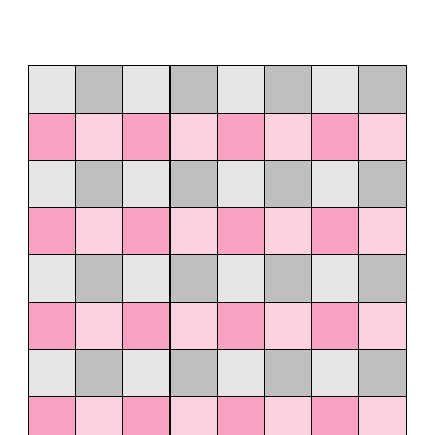
\begin{tikzpicture}[scale=0.6]
			\draw[fill=WildStrawberry, fill opacity=0.4] (0, 0) -- (0, 1) -- (1, 1) -- (1, 0) -- (0, 0);
\draw[fill=WildStrawberry, fill opacity=0.2] (1, 0) -- (1, 1) -- (2, 1) -- (2, 0) -- (1, 0);
\draw[fill=WildStrawberry, fill opacity=0.4] (2, 0) -- (2, 1) -- (3, 1) -- (3, 0) -- (2, 0);
\draw[fill=WildStrawberry, fill opacity=0.2] (3, 0) -- (3, 1) -- (4, 1) -- (4, 0) -- (3, 0);
\draw[fill=WildStrawberry, fill opacity=0.4] (4, 0) -- (4, 1) -- (5, 1) -- (5, 0) -- (4, 0);
\draw[fill=WildStrawberry, fill opacity=0.2] (5, 0) -- (5, 1) -- (6, 1) -- (6, 0) -- (5, 0);
\draw[fill=WildStrawberry, fill opacity=0.4] (6, 0) -- (6, 1) -- (7, 1) -- (7, 0) -- (6, 0);
\draw[fill=WildStrawberry, fill opacity=0.2] (7, 0) -- (7, 1) -- (8, 1) -- (8, 0) -- (7, 0);
\draw[fill=black, fill opacity=0.1] (0, 1) -- (0, 2) -- (1, 2) -- (1, 1) -- (0, 1);
\draw[fill=black, fill opacity=0.25] (1, 1) -- (1, 2) -- (2, 2) -- (2, 1) -- (1, 1);
\draw[fill=black, fill opacity=0.1] (2, 1) -- (2, 2) -- (3, 2) -- (3, 1) -- (2, 1);
\draw[fill=black, fill opacity=0.25] (3, 1) -- (3, 2) -- (4, 2) -- (4, 1) -- (3, 1);
\draw[fill=black, fill opacity=0.1] (4, 1) -- (4, 2) -- (5, 2) -- (5, 1) -- (4, 1);
\draw[fill=black, fill opacity=0.25] (5, 1) -- (5, 2) -- (6, 2) -- (6, 1) -- (5, 1);
\draw[fill=black, fill opacity=0.1] (6, 1) -- (6, 2) -- (7, 2) -- (7, 1) -- (6, 1);
\draw[fill=black, fill opacity=0.25] (7, 1) -- (7, 2) -- (8, 2) -- (8, 1) -- (7, 1);
\draw[fill=WildStrawberry, fill opacity=0.4] (0, 2) -- (0, 3) -- (1, 3) -- (1, 2) -- (0, 2);
\draw[fill=WildStrawberry, fill opacity=0.2] (1, 2) -- (1, 3) -- (2, 3) -- (2, 2) -- (1, 2);
\draw[fill=WildStrawberry, fill opacity=0.4] (2, 2) -- (2, 3) -- (3, 3) -- (3, 2) -- (2, 2);
\draw[fill=WildStrawberry, fill opacity=0.2] (3, 2) -- (3, 3) -- (4, 3) -- (4, 2) -- (3, 2);
\draw[fill=WildStrawberry, fill opacity=0.4] (4, 2) -- (4, 3) -- (5, 3) -- (5, 2) -- (4, 2);
\draw[fill=WildStrawberry, fill opacity=0.2] (5, 2) -- (5, 3) -- (6, 3) -- (6, 2) -- (5, 2);
\draw[fill=WildStrawberry, fill opacity=0.4] (6, 2) -- (6, 3) -- (7, 3) -- (7, 2) -- (6, 2);
\draw[fill=WildStrawberry, fill opacity=0.2] (7, 2) -- (7, 3) -- (8, 3) -- (8, 2) -- (7, 2);
\draw[fill=black, fill opacity=0.1] (0, 3) -- (0, 4) -- (1, 4) -- (1, 3) -- (0, 3);
\draw[fill=black, fill opacity=0.25] (1, 3) -- (1, 4) -- (2, 4) -- (2, 3) -- (1, 3);
\draw[fill=black, fill opacity=0.1] (2, 3) -- (2, 4) -- (3, 4) -- (3, 3) -- (2, 3);
\draw[fill=black, fill opacity=0.25] (3, 3) -- (3, 4) -- (4, 4) -- (4, 3) -- (3, 3);
\draw[fill=black, fill opacity=0.1] (4, 3) -- (4, 4) -- (5, 4) -- (5, 3) -- (4, 3);
\draw[fill=black, fill opacity=0.25] (5, 3) -- (5, 4) -- (6, 4) -- (6, 3) -- (5, 3);
\draw[fill=black, fill opacity=0.1] (6, 3) -- (6, 4) -- (7, 4) -- (7, 3) -- (6, 3);
\draw[fill=black, fill opacity=0.25] (7, 3) -- (7, 4) -- (8, 4) -- (8, 3) -- (7, 3);
\draw[fill=WildStrawberry, fill opacity=0.4] (0, 4) -- (0, 5) -- (1, 5) -- (1, 4) -- (0, 4);
\draw[fill=WildStrawberry, fill opacity=0.2] (1, 4) -- (1, 5) -- (2, 5) -- (2, 4) -- (1, 4);
\draw[fill=WildStrawberry, fill opacity=0.4] (2, 4) -- (2, 5) -- (3, 5) -- (3, 4) -- (2, 4);
\draw[fill=WildStrawberry, fill opacity=0.2] (3, 4) -- (3, 5) -- (4, 5) -- (4, 4) -- (3, 4);
\draw[fill=WildStrawberry, fill opacity=0.4] (4, 4) -- (4, 5) -- (5, 5) -- (5, 4) -- (4, 4);
\draw[fill=WildStrawberry, fill opacity=0.2] (5, 4) -- (5, 5) -- (6, 5) -- (6, 4) -- (5, 4);
\draw[fill=WildStrawberry, fill opacity=0.4] (6, 4) -- (6, 5) -- (7, 5) -- (7, 4) -- (6, 4);
\draw[fill=WildStrawberry, fill opacity=0.2] (7, 4) -- (7, 5) -- (8, 5) -- (8, 4) -- (7, 4);
\draw[fill=black, fill opacity=0.1] (0, 5) -- (0, 6) -- (1, 6) -- (1, 5) -- (0, 5);
\draw[fill=black, fill opacity=0.25] (1, 5) -- (1, 6) -- (2, 6) -- (2, 5) -- (1, 5);
\draw[fill=black, fill opacity=0.1] (2, 5) -- (2, 6) -- (3, 6) -- (3, 5) -- (2, 5);
\draw[fill=black, fill opacity=0.25] (3, 5) -- (3, 6) -- (4, 6) -- (4, 5) -- (3, 5);
\draw[fill=black, fill opacity=0.1] (4, 5) -- (4, 6) -- (5, 6) -- (5, 5) -- (4, 5);
\draw[fill=black, fill opacity=0.25] (5, 5) -- (5, 6) -- (6, 6) -- (6, 5) -- (5, 5);
\draw[fill=black, fill opacity=0.1] (6, 5) -- (6, 6) -- (7, 6) -- (7, 5) -- (6, 5);
\draw[fill=black, fill opacity=0.25] (7, 5) -- (7, 6) -- (8, 6) -- (8, 5) -- (7, 5);
\draw[fill=WildStrawberry, fill opacity=0.4] (0, 6) -- (0, 7) -- (1, 7) -- (1, 6) -- (0, 6);
\draw[fill=WildStrawberry, fill opacity=0.2] (1, 6) -- (1, 7) -- (2, 7) -- (2, 6) -- (1, 6);
\draw[fill=WildStrawberry, fill opacity=0.4] (2, 6) -- (2, 7) -- (3, 7) -- (3, 6) -- (2, 6);
\draw[fill=WildStrawberry, fill opacity=0.2] (3, 6) -- (3, 7) -- (4, 7) -- (4, 6) -- (3, 6);
\draw[fill=WildStrawberry, fill opacity=0.4] (4, 6) -- (4, 7) -- (5, 7) -- (5, 6) -- (4, 6);
\draw[fill=WildStrawberry, fill opacity=0.2] (5, 6) -- (5, 7) -- (6, 7) -- (6, 6) -- (5, 6);
\draw[fill=WildStrawberry, fill opacity=0.4] (6, 6) -- (6, 7) -- (7, 7) -- (7, 6) -- (6, 6);
\draw[fill=WildStrawberry, fill opacity=0.2] (7, 6) -- (7, 7) -- (8, 7) -- (8, 6) -- (7, 6);
\draw[fill=black, fill opacity=0.1] (0, 7) -- (0, 8) -- (1, 8) -- (1, 7) -- (0, 7);
\draw[fill=black, fill opacity=0.25] (1, 7) -- (1, 8) -- (2, 8) -- (2, 7) -- (1, 7);
\draw[fill=black, fill opacity=0.1] (2, 7) -- (2, 8) -- (3, 8) -- (3, 7) -- (2, 7);
\draw[fill=black, fill opacity=0.25] (3, 7) -- (3, 8) -- (4, 8) -- (4, 7) -- (3, 7);
\draw[fill=black, fill opacity=0.1] (4, 7) -- (4, 8) -- (5, 8) -- (5, 7) -- (4, 7);
\draw[fill=black, fill opacity=0.25] (5, 7) -- (5, 8) -- (6, 8) -- (6, 7) -- (5, 7);
\draw[fill=black, fill opacity=0.1] (6, 7) -- (6, 8) -- (7, 8) -- (7, 7) -- (6, 7);
\draw[fill=black, fill opacity=0.25] (7, 7) -- (7, 8) -- (8, 8) -- (8, 7) -- (7, 7);
		\end{tikzpicture}
	\end{center}
	\caption{Six regions that each define a binary bit via the parity of the number of heads-up coins in the squares highlighted in red.}
	\label{fig:TheChessboardEncodingProblem_Grids}
\end{figure}

In the example shown in figure~\ref{fig:TheChessboardEncodingProblem_Example} the key has been hidden in fourth row and third column. Using the first three digits to encode the column number and the last three digits to encode the row number, this is encoded as 011100. In the red highlighted region in figure~\ref{fig:TheChessboardEncodingProblem_1} there are 16 heads which is equal to 0 modulo 2. This matches the first digit in the number we want to encode which means we want to preserve the parity of heads in this region, therefore we will flip a coin outside the red highlighted region, that is, on the left. We can do a similar process for the other regions and this is described in table~\ref{tab:TheChessboardEncodingProblem_ExampleParity}

\begin{figure}[H]
	\centering
	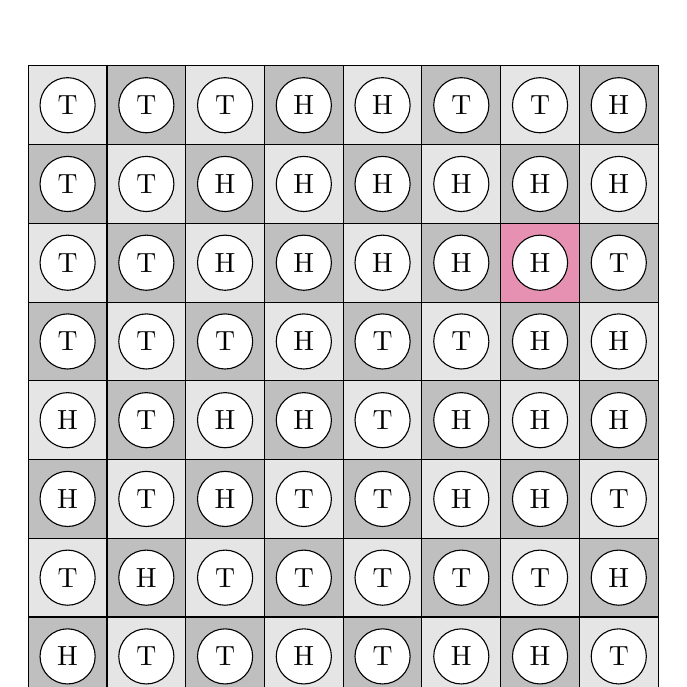
\begin{tikzpicture}[scale=1]
		\draw[fill=black, fill opacity=0.25] (0, 0) -- (0, 1) -- (1, 1) -- (1, 0) -- (0, 0);
\draw[fill=black, fill opacity=0.1] (1, 0) -- (1, 1) -- (2, 1) -- (2, 0) -- (1, 0);
\draw[fill=black, fill opacity=0.25] (2, 0) -- (2, 1) -- (3, 1) -- (3, 0) -- (2, 0);
\draw[fill=black, fill opacity=0.1] (3, 0) -- (3, 1) -- (4, 1) -- (4, 0) -- (3, 0);
\draw[fill=black, fill opacity=0.25] (4, 0) -- (4, 1) -- (5, 1) -- (5, 0) -- (4, 0);
\draw[fill=black, fill opacity=0.1] (5, 0) -- (5, 1) -- (6, 1) -- (6, 0) -- (5, 0);
\draw[fill=black, fill opacity=0.25] (6, 0) -- (6, 1) -- (7, 1) -- (7, 0) -- (6, 0);
\draw[fill=black, fill opacity=0.1] (7, 0) -- (7, 1) -- (8, 1) -- (8, 0) -- (7, 0);
\draw[fill=black, fill opacity=0.1] (0, 1) -- (0, 2) -- (1, 2) -- (1, 1) -- (0, 1);
\draw[fill=black, fill opacity=0.25] (1, 1) -- (1, 2) -- (2, 2) -- (2, 1) -- (1, 1);
\draw[fill=black, fill opacity=0.1] (2, 1) -- (2, 2) -- (3, 2) -- (3, 1) -- (2, 1);
\draw[fill=black, fill opacity=0.25] (3, 1) -- (3, 2) -- (4, 2) -- (4, 1) -- (3, 1);
\draw[fill=black, fill opacity=0.1] (4, 1) -- (4, 2) -- (5, 2) -- (5, 1) -- (4, 1);
\draw[fill=black, fill opacity=0.25] (5, 1) -- (5, 2) -- (6, 2) -- (6, 1) -- (5, 1);
\draw[fill=black, fill opacity=0.1] (6, 1) -- (6, 2) -- (7, 2) -- (7, 1) -- (6, 1);
\draw[fill=black, fill opacity=0.25] (7, 1) -- (7, 2) -- (8, 2) -- (8, 1) -- (7, 1);
\draw[fill=black, fill opacity=0.25] (0, 2) -- (0, 3) -- (1, 3) -- (1, 2) -- (0, 2);
\draw[fill=black, fill opacity=0.1] (1, 2) -- (1, 3) -- (2, 3) -- (2, 2) -- (1, 2);
\draw[fill=black, fill opacity=0.25] (2, 2) -- (2, 3) -- (3, 3) -- (3, 2) -- (2, 2);
\draw[fill=black, fill opacity=0.1] (3, 2) -- (3, 3) -- (4, 3) -- (4, 2) -- (3, 2);
\draw[fill=black, fill opacity=0.25] (4, 2) -- (4, 3) -- (5, 3) -- (5, 2) -- (4, 2);
\draw[fill=black, fill opacity=0.1] (5, 2) -- (5, 3) -- (6, 3) -- (6, 2) -- (5, 2);
\draw[fill=black, fill opacity=0.25] (6, 2) -- (6, 3) -- (7, 3) -- (7, 2) -- (6, 2);
\draw[fill=black, fill opacity=0.1] (7, 2) -- (7, 3) -- (8, 3) -- (8, 2) -- (7, 2);
\draw[fill=black, fill opacity=0.1] (0, 3) -- (0, 4) -- (1, 4) -- (1, 3) -- (0, 3);
\draw[fill=black, fill opacity=0.25] (1, 3) -- (1, 4) -- (2, 4) -- (2, 3) -- (1, 3);
\draw[fill=black, fill opacity=0.1] (2, 3) -- (2, 4) -- (3, 4) -- (3, 3) -- (2, 3);
\draw[fill=black, fill opacity=0.25] (3, 3) -- (3, 4) -- (4, 4) -- (4, 3) -- (3, 3);
\draw[fill=black, fill opacity=0.1] (4, 3) -- (4, 4) -- (5, 4) -- (5, 3) -- (4, 3);
\draw[fill=black, fill opacity=0.25] (5, 3) -- (5, 4) -- (6, 4) -- (6, 3) -- (5, 3);
\draw[fill=black, fill opacity=0.1] (6, 3) -- (6, 4) -- (7, 4) -- (7, 3) -- (6, 3);
\draw[fill=black, fill opacity=0.25] (7, 3) -- (7, 4) -- (8, 4) -- (8, 3) -- (7, 3);
\draw[fill=black, fill opacity=0.25] (0, 4) -- (0, 5) -- (1, 5) -- (1, 4) -- (0, 4);
\draw[fill=black, fill opacity=0.1] (1, 4) -- (1, 5) -- (2, 5) -- (2, 4) -- (1, 4);
\draw[fill=black, fill opacity=0.25] (2, 4) -- (2, 5) -- (3, 5) -- (3, 4) -- (2, 4);
\draw[fill=black, fill opacity=0.1] (3, 4) -- (3, 5) -- (4, 5) -- (4, 4) -- (3, 4);
\draw[fill=black, fill opacity=0.25] (4, 4) -- (4, 5) -- (5, 5) -- (5, 4) -- (4, 4);
\draw[fill=black, fill opacity=0.1] (5, 4) -- (5, 5) -- (6, 5) -- (6, 4) -- (5, 4);
\draw[fill=black, fill opacity=0.25] (6, 4) -- (6, 5) -- (7, 5) -- (7, 4) -- (6, 4);
\draw[fill=black, fill opacity=0.1] (7, 4) -- (7, 5) -- (8, 5) -- (8, 4) -- (7, 4);
\draw[fill=black, fill opacity=0.1] (0, 5) -- (0, 6) -- (1, 6) -- (1, 5) -- (0, 5);
\draw[fill=black, fill opacity=0.25] (1, 5) -- (1, 6) -- (2, 6) -- (2, 5) -- (1, 5);
\draw[fill=black, fill opacity=0.1] (2, 5) -- (2, 6) -- (3, 6) -- (3, 5) -- (2, 5);
\draw[fill=black, fill opacity=0.25] (3, 5) -- (3, 6) -- (4, 6) -- (4, 5) -- (3, 5);
\draw[fill=black, fill opacity=0.1] (4, 5) -- (4, 6) -- (5, 6) -- (5, 5) -- (4, 5);
\draw[fill=black, fill opacity=0.25] (5, 5) -- (5, 6) -- (6, 6) -- (6, 5) -- (5, 5);
\draw[fill=black, fill opacity=0.1] (6, 5) -- (6, 6) -- (7, 6) -- (7, 5) -- (6, 5);
\draw[fill=black, fill opacity=0.25] (7, 5) -- (7, 6) -- (8, 6) -- (8, 5) -- (7, 5);
\draw[fill=black, fill opacity=0.25] (0, 6) -- (0, 7) -- (1, 7) -- (1, 6) -- (0, 6);
\draw[fill=black, fill opacity=0.1] (1, 6) -- (1, 7) -- (2, 7) -- (2, 6) -- (1, 6);
\draw[fill=black, fill opacity=0.25] (2, 6) -- (2, 7) -- (3, 7) -- (3, 6) -- (2, 6);
\draw[fill=black, fill opacity=0.1] (3, 6) -- (3, 7) -- (4, 7) -- (4, 6) -- (3, 6);
\draw[fill=black, fill opacity=0.25] (4, 6) -- (4, 7) -- (5, 7) -- (5, 6) -- (4, 6);
\draw[fill=black, fill opacity=0.1] (5, 6) -- (5, 7) -- (6, 7) -- (6, 6) -- (5, 6);
\draw[fill=black, fill opacity=0.25] (6, 6) -- (6, 7) -- (7, 7) -- (7, 6) -- (6, 6);
\draw[fill=black, fill opacity=0.1] (7, 6) -- (7, 7) -- (8, 7) -- (8, 6) -- (7, 6);
\draw[fill=black, fill opacity=0.1] (0, 7) -- (0, 8) -- (1, 8) -- (1, 7) -- (0, 7);
\draw[fill=black, fill opacity=0.25] (1, 7) -- (1, 8) -- (2, 8) -- (2, 7) -- (1, 7);
\draw[fill=black, fill opacity=0.1] (2, 7) -- (2, 8) -- (3, 8) -- (3, 7) -- (2, 7);
\draw[fill=black, fill opacity=0.25] (3, 7) -- (3, 8) -- (4, 8) -- (4, 7) -- (3, 7);
\draw[fill=black, fill opacity=0.1] (4, 7) -- (4, 8) -- (5, 8) -- (5, 7) -- (4, 7);
\draw[fill=black, fill opacity=0.25] (5, 7) -- (5, 8) -- (6, 8) -- (6, 7) -- (5, 7);
\draw[fill=black, fill opacity=0.1] (6, 7) -- (6, 8) -- (7, 8) -- (7, 7) -- (6, 7);
\draw[fill=black, fill opacity=0.25] (7, 7) -- (7, 8) -- (8, 8) -- (8, 7) -- (7, 7);

\draw[fill=WildStrawberry, fill opacity=0.4] (6, 5) -- (6, 6) -- (7, 6) -- (7, 5) -- (6, 5);

\draw[fill=white, fill opacity=1](0.5, 0.5) circle (0.35);
\node at (0.5, 0.5) {H};
\draw[fill=white, fill opacity=1](1.5, 0.5) circle (0.35);
\node at (1.5, 0.5) {T};
\draw[fill=white, fill opacity=1](2.5, 0.5) circle (0.35);
\node at (2.5, 0.5) {T};
\draw[fill=white, fill opacity=1](3.5, 0.5) circle (0.35);
\node at (3.5, 0.5) {H};
\draw[fill=white, fill opacity=1](4.5, 0.5) circle (0.35);
\node at (4.5, 0.5) {T};
\draw[fill=white, fill opacity=1](5.5, 0.5) circle (0.35);
\node at (5.5, 0.5) {H};
\draw[fill=white, fill opacity=1](6.5, 0.5) circle (0.35);
\node at (6.5, 0.5) {H};
\draw[fill=white, fill opacity=1](7.5, 0.5) circle (0.35);
\node at (7.5, 0.5) {T};
\draw[fill=white, fill opacity=1](0.5, 1.5) circle (0.35);
\node at (0.5, 1.5) {T};
\draw[fill=white, fill opacity=1](1.5, 1.5) circle (0.35);
\node at (1.5, 1.5) {H};
\draw[fill=white, fill opacity=1](2.5, 1.5) circle (0.35);
\node at (2.5, 1.5) {T};
\draw[fill=white, fill opacity=1](3.5, 1.5) circle (0.35);
\node at (3.5, 1.5) {T};
\draw[fill=white, fill opacity=1](4.5, 1.5) circle (0.35);
\node at (4.5, 1.5) {T};
\draw[fill=white, fill opacity=1](5.5, 1.5) circle (0.35);
\node at (5.5, 1.5) {T};
\draw[fill=white, fill opacity=1](6.5, 1.5) circle (0.35);
\node at (6.5, 1.5) {T};
\draw[fill=white, fill opacity=1](7.5, 1.5) circle (0.35);
\node at (7.5, 1.5) {H};
\draw[fill=white, fill opacity=1](0.5, 2.5) circle (0.35);
\node at (0.5, 2.5) {H};
\draw[fill=white, fill opacity=1](1.5, 2.5) circle (0.35);
\node at (1.5, 2.5) {T};
\draw[fill=white, fill opacity=1](2.5, 2.5) circle (0.35);
\node at (2.5, 2.5) {H};
\draw[fill=white, fill opacity=1](3.5, 2.5) circle (0.35);
\node at (3.5, 2.5) {T};
\draw[fill=white, fill opacity=1](4.5, 2.5) circle (0.35);
\node at (4.5, 2.5) {T};
\draw[fill=white, fill opacity=1](5.5, 2.5) circle (0.35);
\node at (5.5, 2.5) {H};
\draw[fill=white, fill opacity=1](6.5, 2.5) circle (0.35);
\node at (6.5, 2.5) {H};
\draw[fill=white, fill opacity=1](7.5, 2.5) circle (0.35);
\node at (7.5, 2.5) {T};
\draw[fill=white, fill opacity=1](0.5, 3.5) circle (0.35);
\node at (0.5, 3.5) {H};
\draw[fill=white, fill opacity=1](1.5, 3.5) circle (0.35);
\node at (1.5, 3.5) {T};
\draw[fill=white, fill opacity=1](2.5, 3.5) circle (0.35);
\node at (2.5, 3.5) {H};
\draw[fill=white, fill opacity=1](3.5, 3.5) circle (0.35);
\node at (3.5, 3.5) {H};
\draw[fill=white, fill opacity=1](4.5, 3.5) circle (0.35);
\node at (4.5, 3.5) {T};
\draw[fill=white, fill opacity=1](5.5, 3.5) circle (0.35);
\node at (5.5, 3.5) {H};
\draw[fill=white, fill opacity=1](6.5, 3.5) circle (0.35);
\node at (6.5, 3.5) {H};
\draw[fill=white, fill opacity=1](7.5, 3.5) circle (0.35);
\node at (7.5, 3.5) {H};
\draw[fill=white, fill opacity=1](0.5, 4.5) circle (0.35);
\node at (0.5, 4.5) {T};
\draw[fill=white, fill opacity=1](1.5, 4.5) circle (0.35);
\node at (1.5, 4.5) {T};
\draw[fill=white, fill opacity=1](2.5, 4.5) circle (0.35);
\node at (2.5, 4.5) {T};
\draw[fill=white, fill opacity=1](3.5, 4.5) circle (0.35);
\node at (3.5, 4.5) {H};
\draw[fill=white, fill opacity=1](4.5, 4.5) circle (0.35);
\node at (4.5, 4.5) {T};
\draw[fill=white, fill opacity=1](5.5, 4.5) circle (0.35);
\node at (5.5, 4.5) {T};
\draw[fill=white, fill opacity=1](6.5, 4.5) circle (0.35);
\node at (6.5, 4.5) {H};
\draw[fill=white, fill opacity=1](7.5, 4.5) circle (0.35);
\node at (7.5, 4.5) {H};
\draw[fill=white, fill opacity=1](0.5, 5.5) circle (0.35);
\node at (0.5, 5.5) {T};
\draw[fill=white, fill opacity=1](1.5, 5.5) circle (0.35);
\node at (1.5, 5.5) {T};
\draw[fill=white, fill opacity=1](2.5, 5.5) circle (0.35);
\node at (2.5, 5.5) {H};
\draw[fill=white, fill opacity=1](3.5, 5.5) circle (0.35);
\node at (3.5, 5.5) {H};
\draw[fill=white, fill opacity=1](4.5, 5.5) circle (0.35);
\node at (4.5, 5.5) {H};
\draw[fill=white, fill opacity=1](5.5, 5.5) circle (0.35);
\node at (5.5, 5.5) {H};
\draw[fill=white, fill opacity=1](6.5, 5.5) circle (0.35);
\node at (6.5, 5.5) {H};
\draw[fill=white, fill opacity=1](7.5, 5.5) circle (0.35);
\node at (7.5, 5.5) {T};
\draw[fill=white, fill opacity=1](0.5, 6.5) circle (0.35);
\node at (0.5, 6.5) {T};
\draw[fill=white, fill opacity=1](1.5, 6.5) circle (0.35);
\node at (1.5, 6.5) {T};
\draw[fill=white, fill opacity=1](2.5, 6.5) circle (0.35);
\node at (2.5, 6.5) {H};
\draw[fill=white, fill opacity=1](3.5, 6.5) circle (0.35);
\node at (3.5, 6.5) {H};
\draw[fill=white, fill opacity=1](4.5, 6.5) circle (0.35);
\node at (4.5, 6.5) {H};
\draw[fill=white, fill opacity=1](5.5, 6.5) circle (0.35);
\node at (5.5, 6.5) {H};
\draw[fill=white, fill opacity=1](6.5, 6.5) circle (0.35);
\node at (6.5, 6.5) {H};
\draw[fill=white, fill opacity=1](7.5, 6.5) circle (0.35);
\node at (7.5, 6.5) {H};
\draw[fill=white, fill opacity=1](0.5, 7.5) circle (0.35);
\node at (0.5, 7.5) {T};
\draw[fill=white, fill opacity=1](1.5, 7.5) circle (0.35);
\node at (1.5, 7.5) {T};
\draw[fill=white, fill opacity=1](2.5, 7.5) circle (0.35);
\node at (2.5, 7.5) {T};
\draw[fill=white, fill opacity=1](3.5, 7.5) circle (0.35);
\node at (3.5, 7.5) {H};
\draw[fill=white, fill opacity=1](4.5, 7.5) circle (0.35);
\node at (4.5, 7.5) {H};
\draw[fill=white, fill opacity=1](5.5, 7.5) circle (0.35);
\node at (5.5, 7.5) {T};
\draw[fill=white, fill opacity=1](6.5, 7.5) circle (0.35);
\node at (6.5, 7.5) {T};
\draw[fill=white, fill opacity=1](7.5, 7.5) circle (0.35);
\node at (7.5, 7.5) {H};
	\end{tikzpicture}
	\caption{An example of random coins on a chessboard. The red highlighted square indicates the position of the key.}
	\label{fig:TheChessboardEncodingProblem_Example}
\end{figure}

\begin{table}[H]
	\centering
	\caption{An example of how to determine which regions to flip the parity of}
	\label{tab:TheChessboardEncodingProblem_ExampleParity}
	\begin{tabular}{cccccc}
		\myhline
		Region & Head Count & Head Parity & Encoded Parity & Parity Change & Flip Red Region  \\
		\myhline
		\tableinput{1 - Logic/TheChessboardEncodingProblem/ChessboardExampleTable.tex}
		\myhline
	\end{tabular}
\end{table}

\textbf{Extensions and Comments:}
\newpage
\subsection{Pills While Blindfolded}

This a nice and accessible problem that requires some out of the box thinking. Good problem for when walking as paper would not help much. I give this problem a 1/10 in difficulty.

An evil logician has poisoned you, but gives you a way to survive. They offer you two red pills and two blue pills and to survive you need to take exactly one red and one blue pill. The only complication is that you are blindfolded. What is your strategy to survive? Standard evil logician rules apply.

\textbf{Hints:}

\begin{enumerate}
	\item There is no way to gain any information about what colour the pills are. This means your strategy would have to work for any permutation of the pills.
	\item Taking all the pills would give you exactly double the dose.
	\item Consider the same problem but with one red pill and one blue pill and needing to take half of each. Apply this to the problem with four pills.
\end{enumerate}

\textbf{Solution:}

Arrange all the pills in a line, such as ``O O O O". Instead of splitting them vertically down the middle like ``O O $|$ O O", cut them horizontally. Each half will contain exactly two lots of half a red pill and two lots of half a blue pill. This is the same amount as one red pill and one blue pill.

\textbf{Extensions and Comments:}

It is not stated whether you can or cannot cut the pills in the problems statement, but I think if you gave this information it would completely give away the solution. I think it is better to leave this as the creative option. This problem works with any number of pills and any number of colour of pills.\newpage

\stopcontents\newpage
\section{Numbers}

\thispagestyle{subcontents}

\vspace{-5mm}
\startcontents
\printcontents{}{1}{\section*{\contentsname}}
\clearpage

% Date added: 12/09/2024

\subsection{Six Digit And Two Set Comparison}

I found this problem in a book of problems from the Grade Five Leningrad Mathematical Olympiad~\cite{Grade5LeningradOlympiad}, in particular, this is question two from 1989. I have only found one person who could solve this as of 2024 so it may be trickier than it seems given it is designed for 11 year old children.

Consider the set of six digit numbers including leading zeros, that is, 000000 to 999999. Set $X$ is defined as all such numbers where the first three digits sum to the same amount as the sum of the last three digits. Set $Y$ is defined as all such numbers where all the digits add up to 27. Show that sets $X$ and $Y$ are the same size.

\textbf{Hints:}

\begin{enumerate}
    \item The size of each set does not need to be determined.
    \item The fact that $27 = 3 \cdot 9 = \frac{6}{2} \cdot (\text{base} - 1)$ is not a coincidence.
    \item Make a bijection between the sets.
\end{enumerate}

\textbf{Solution:}

Denote the number as the concatenation of six digits, $abcABC$, and using the same notation consider the map $\phi(abcABC) = (9 - a)(9 - b)(9 - c)ABC$. Intuitively it can be seen that $\phi$ uniquely pairs up numbers between the two sets, meaning that they must be the same size as otherwise one set would not be big enough to produce pairs for the other set.

To prove this, it is shown that $\phi$ is a bijective involution between the sets, implying that they are the same size. First we see that $\phi$ is well-defined, as each digit from 0 to 9 is mapped to another digit from 0 to 9. Therefore the result of applying $\phi$ to a six digit base ten number is another six digit base ten number, and each digit in the input only affects the digit in the same position in the output. The following implications show that $\phi$ maps $X$ to $Y$.

\begin{align*}
    & abcABC \in X  \\
    \iff & a + b + c = A + B + C  \\
    \iff & 27 = (9 - a) + (9 - b) + (9 - c) + A + B + C  \\
    \iff & 27 = \text{Digit sum}(\phi(abcABC))  \\
    \iff & \phi(abcABC) \in Y
\end{align*}

It is clear that $\phi(\phi(abcABC)) = abcABC$. This implies that it is impossible for $\phi$ to map two distinct inputs to the same output, as otherwise $\phi$ would need to map that result to both inputs simultaneously. This also implies that every six digit number must be in the image of $\phi$, meaning the reverse implications presented previously combined with $\phi^2$ being the identity map implies that $\phi$ maps $Y$ to $X$. Together this shows that $X$ and $Y$ are at least as large as each other, and therefore the same size.

\textbf{Extensions and Comments:}

A similar problem can be given in any base, and for any even number of digits with a near identical proof. I like this problem because it uses a way of understanding size that is very fundamental, but people do not usually think about. The size of each set does not need to be determined, but it can be found by taking square of the number of occurrences for each unique digit sum, and adding together. This gives 55252 as the size of $X$ and $Y$.

The relationship between the sums of the first and last three digits and the total sum is actually much closer than this problem suggests. In the notation used previously, define the difference to be $A + B +C - a - b -c$, and the total to be the digit sum. Define $X_d$ to be the set of numbers that have the same difference, and define $Y_t$ to be the set of numbers that have the same total. Almost identical reasoning used to solve this puzzle can be used to show that $|X_{d-27}| = |Y_t|$. Additionally, a map that subtracts each digit from 9 can be used to show that $|X_d| = |X_{-d}|$ and $|Y_t| = |Y_{54 - t}|$. This property extends to other bases and other even number of digits, and is demonstrated explicitly in table~\ref{tab:SixDigitAndTwoSetComparison}.

\begin{table}[H]
    \centering
    \caption{The distribution of the size of $X_d$ and $Y_t$}
    \label{tab:SixDigitAndTwoSetComparison}
    \begin{tabular}{cc@{\hspace{12mm}}cc}
        \myhline
        \multicolumn{2}{c@{\hspace{12mm}}}{Difference} & \multicolumn{2}{c@{\hspace{6mm}}}{Total}  \\
        Value & Count & Value & Count  \\
        \myhline
        -27 &     1 &     0 &     1  \\
        -26 &     6 &     1 &     6  \\
        -25 &    21 &     2 &    21  \\
        -24 &    56 &     3 &    56  \\
        -23 &   126 &     4 &   126  \\
        -22 &   252 &     5 &   252  \\
        -21 &   462 &     6 &   462  \\
        -20 &   792 &     7 &   792  \\
        -19 &  1287 &     8 &  1287  \\
        -18 &  2002 &     9 &  2002  \\
        -17 &  2997 &    10 &  2997  \\
        -16 &  4332 &    11 &  4332  \\
        -15 &  6062 &    12 &  6062  \\
        -14 &  8232 &    13 &  8232  \\
        -13 & 10872 &    14 & 10872  \\
        -12 & 13992 &    15 & 13992  \\
        -11 & 17577 &    16 & 17577  \\
        -10 & 21582 &    17 & 21582  \\
         -9 & 25927 &    18 & 25927  \\
         -8 & 30492 &    19 & 30492  \\
         -7 & 35127 &    20 & 35127  \\
         -6 & 39662 &    21 & 39662  \\
         -5 & 43917 &    22 & 43917  \\
         -4 & 47712 &    23 & 47712  \\
         -3 & 50877 &    24 & 50877  \\
         -2 & 53262 &    25 & 53262  \\
         -1 & 54747 &    26 & 54747  \\
          0 & 55252 &    27 & 55252  \\
          1 & 54747 &    28 & 54747  \\
          2 & 53262 &    29 & 53262  \\
          3 & 50877 &    30 & 50877  \\
          4 & 47712 &    31 & 47712  \\
          5 & 43917 &    32 & 43917  \\
          6 & 39662 &    33 & 39662  \\
          7 & 35127 &    34 & 35127  \\
          8 & 30492 &    35 & 30492  \\
          9 & 25927 &    36 & 25927  \\
         10 & 21582 &    37 & 21582  \\
         11 & 17577 &    38 & 17577  \\
         12 & 13992 &    39 & 13992  \\
         13 & 10872 &    40 & 10872  \\
         14 &  8232 &    41 &  8232  \\
         15 &  6062 &    42 &  6062  \\
        \myhline
    \end{tabular}
\end{table}
\newpage
\subsection{Appending Cyclicly Mapped Sequence}

This problem was part of the coding assessment for Blackrock which I was helping a friend with. I originally did this in the naive way as I had the power of Python, but looking at it further I realised there was a simple solution. This puzzle does not require any large leaps in understanding and the solution builds quite naturally. I consider this problem a 4/10 in terms of difficulty.

At the 0$^\text{th}$ iteration, a sequence is the single digit 0. On each iteration, all zeros are mapped to one, all ones are mapped to two, and all twos are mapped to zero. The transformed sequence is then appended on to the end of the original sequence to get the sequence for the next iteration. The question is to find a nice method or expression to determine the value of the digit at index $n$ where the first digit is defined to be at index 0. The first few terms are shown below.

\begin{center}
    0  \\
    01  \\
    0112  \\
    01121220  \\
    0112122012202002
\end{center}

\textbf{Hints:}

\begin{enumerate}
    \item It is not necessary to generate the whole sequence.
    \item Initially forget about taking the result modulo 3, and assume a base with infinitely many symbols.
    \item Convert $n$ to binary.
\end{enumerate}

\textbf{Solution:}

The digit sum of the binary digits of $n$ modulo 3 gives the answer. At any given iteration, an index is either part of the original sequence in the previous iteration, or is part of the appended sequence. The digit would have had one added to it modulo three at an iteration if and only if it was in the appended part at that iteration, and therefore the history of each position should be understood.

Take $13$ as an example. At the fourth iteration, it is in the appended part as it is larger than $8$. The mapped digit was $13 - 8 = 5$. At the third iteration this index was also in the appended part as it is larger than $4$, and the mapped digit was $1$. This was in the original part of the sequence at the second iteration, and in the appended part at the first iteration. Going from the last iteration backwards gives a history of appended, appended, original, appended, matching the binary expansion, $1101$.

To see this relationship with the binary more generally, note that at iteration $n$, the index $k$ is in the appended part if and only if the $k \ \text{mod} \ 2^{n-1}$ index is in the appended part. This is the case if and only if the $n^\text{th}$ binary digit of $k$ is $1$, as the binary expansion of $k \ \text{mod} \ 2^{n-1}$ is the same as that of $k$ but truncated to leave the last $n$ digits. To get the digit at the $k^\text{th}$ position, it is only necessary to find the number of times it was in the appended part as this is the number of times a 1 was added to it. This corresponds exactly to the sum of the digits in the binary expansion of $k$, and $\text{mod}$ commutes with addition, therefore the modulus can be taken after the sum.

\textbf{Extensions and Comments:}

This solution builds quite naturally and an initial approach of testing some examples does well to give an intuition as to how the problem works. I think this would work better as a supervised interview question instead of as a coding test as there is nice problem solving here. The only line of Python code needed is \texttt{sum([int(i) for i in bin(n)[2:]]) \% 3}. This problem easily extends for transformation rules that use addition of any constant modulo any other positive natural number by the same argument, although with the extra step of multiplying the sum of binary digits by the constant added to the appended part. The time and memory complexity of the solution offered here is $O(\log n)$, whereas the naive method of generating the whole sequence needed and selecting the digit has a complexity of $O(n)$.

\subsection{5 by 6 Magic Rectangle}

This is question 1 from the 1979 Grade 5 Leningrad Mathematical Olympiad~\cite{Grade5LeningradOlympiad}, so it was designed for children aged around 11. Despite this, most people I ask have not been able to solve it and give up very quickly. Personally I think the success rate would be higher if people were more tenacious, and I give this problem a difficulty of 2/10.

The numbers 1 to 30 are each to be placed in a 5 by 6 grid without repeats such that all the rows sum to the same total, and all the columns sum to the same total. Determine whether this is possible, and if so, provide a solution.

\textbf{Hints:}

\begin{enumerate}
	\item Be more systematic than trying to move the numbers around to get the same totals.
	\item Think about how you would calculate the totals for the rows and columns.
\end{enumerate}

This problem becomes easy when you think about it systematically. Before placing any numbers in the table, the totals for the rows and columns should be found as a target to aim for. The sum of all the column totals will be equal to the sum of all the numbers in the grid, and similarly for the rows. This total is an invariant of the problem, any arrangement of numbers will give the same total sum. This invariant can be determined using the formula for the sum of the first $n$ natural numbers, giving $S = \frac{1}{2} \cdot 30 \cdot 31 = 15 \cdot 31$. As the column total is a constant, the sum of the column totals will be a multiple of 6 as there are six columns. This means the sum of all numbers in the grid is also a multiple of 6. $S = 15 \cdot 31$, which are both odd, therefore the column total cannot be a whole number. As the column total is the sum of whole numbers, this is a contradiction, and the task is impossible.

\textbf{Extensions and Comments:}

This method will show that such a grid is impossible if and only if the dimensions of the grid are of different parities. This can be done by substituting general odd and even numbers into the formula $\frac{1}{2} \cdot nm  \cdot (nm + 1)$. In the case of two even number or two odd numbers, the expression can be expanded and divided by either of the numbers to get a whole number. In the case of one number being even and the other being odd, it can be seen that dividing the expression by the even number gives $\frac{1}{2} \cdot \text{ODD} \cdot {\text{EVEN} + 1}$ which cannot be an integer (THIS IS INCORRECT, FIX THIS). Passing this test does not imply that such a magic rectangle is possible however, for example there are only two possible 2 by 2 grids and neither of them are magic.\newpage
\subsection{Irrational to High Power Near Integer}

This problem was given to me by my Oxford admissions preparation tutor, Jeremy. The original problem he gave was ``what happens, now prove it", where I found the first part, and which I have decided to reveal upfront. I came back to this problem in 2024 and solved it in around 20 minutes and I have provided this proof as the second solution. Dr Barker on YouTube also covered this problem and gave the much slicker argument which is given as the first solution. This problem benefits greatly from pen and paper, and is much more suited to the mathematically inclined. I rate this problem a 5 out of 10 in terms of difficulty.

$(1 + \sqrt{2})^n$ gets close to an integer when raised to a high power. Explain why this is the case. Extension question: characterise exactly which $a + \sqrt{b}$ where this occurs.

\textbf{Hints for Solution 1:}

\begin{enumerate}
    \item Use the binomial expansion to expand $\left( 1 + \sqrt{2} \right)^n$. How would you need to modify this to make the odd powers of $\sqrt{2}$ disappear?
    \item Consider the conjugate, $\left( 1 - \sqrt{2} \right)^n$.
    \item Add the conjugate to the original to make the odd powers cancel out.
\end{enumerate}

\textbf{Solution 1:}

We define $a_n = \left( 1 + \sqrt{2} \right)^n$ and $b_n$ as the sum of $\left (1 + \sqrt{2} \right)^n$ and its conjugate. Using the binomial expansion we see in equation~\eqref{eqn:IrrationalToHighPowerNearInteger} that the odd powers of $\sqrt{2}$ cancel out, and thus $b_n$ is an integer. We also note that $\left| 1 - \sqrt{2} \right| < 1$, and therefore it annihilates when raising it to increasingly higher powers. This means $|a_n - b_n| \to 0$ as $n \to \infty$, and thus $a_n$ converges to an integer.

\begin{align}
	\begin{split}
		b_n &= \left( 1 + \sqrt{2} \right)^n + \left( 1 - \sqrt{2} \right)^n  \\
		&= \sum_{k=0}^n {n \choose k} \left( 1^{n - k} \cdot \sqrt{2}^k + 1^{n - k} \cdot (-\sqrt{2})^k \right)  \\
		&= \sum_{k=0}^n {n \choose k} \sqrt{2}^k \cdot (1 + (-1)^k)  \\
		&= \sum_{k=0}^n {n \choose k} \sqrt{2}^k \cdot \{k \ \text{is even}\}  \\
		&= \sum_{m=0}^{\left\lfloor \frac{n}{2} \right\rfloor} {n \choose 2m} 2^m \in \mathbb{N}
		\label{eqn:IrrationalToHighPowerNearInteger}
	\end{split}	
\end{align}

\textbf{Hints for Solution 2:}

\begin{enumerate}
    \item 
\end{enumerate}

\textbf{Solution 2:}



\textbf{Extensions and Comments:}\newpage
\subsection{Spherical Polar Basis}

\textbf{Hints:}

\begin{enumerate}
    \item 
\end{enumerate}

\textbf{Solution:}



\textbf{Extensions and Comments:}\newpage
\subsection{Interpolating Polynomials}

This subsection is about a series of results I found about interpolating polynomials that are all linked together. I found these at several different points throughout my mathematical journey, and have attempted to present them in a way that highlights how one might discover them for themselves.

\subsubsection{Calculus of Differences and $n^\text{th}$ Term Rule}

The $n^\text{th}$ term rule is a function from the natural numbers excluding 0 to the reals that generates a sequence. In year 9 we were shown a method to find the $n^\text{th}$ term rule for a sequence generated by a quadratic polynomial that confused me, and when I investigated this for myself I found an extension to higher orders. I did not prove that this always worked at the time, and did so when I revisited the topic during my maths masters. Determining a cubic polynomial for a four term sequence was one of the very first programs I wrote soon after I turned 15. During the winter holiday I wrote a version that could find the polynomial for arbitrary length sequences.



\subsubsection{The Lagrange Interpolating Polynomial}

In my second year of undergrad I was doing problem sheet 1 from part A linear algebra~\cite{PartALinearAlgebraSheet1}, and question two was the following.

\begin{center}
    (Harder) Show that the space of functions $f : \mathbb{N} \to \mathbb{R}$ does not have a countable basis.
\end{center}

I was not initially convinced by this and thought that a polynomial interpolating all the points of $f$ would be a counterexample. I have discussed why this reasoning is wrong in the extensions and comments, along with the answer to the original question. I am also not sure why I did not realise I had my supposed counterexample from the calculus of differences method, but nonetheless I found a new method that is the subject of this exercise. If I was a teacher then I would definitely be giving this problem to my students.

Given a finite set, $A \subset \mathbb{R}$, and a function $f : A \to \mathbb{R}$, find an  interpolating polynomial of lowest degree, $p : A \to \mathbb{R}$. That is $f(x_i) = p(x_i) \quad \forall x_i \in A$. This is known as the Lagrange Interpolating Polynomial, or simply the Lagrange Polynomial. Finding an explicit formula is the first part of the question, and showing it is minimal is the second part.

\textbf{Hints:}

\begin{enumerate}
    \item Use linearity - the finite sum of a collection of polynomials is also a polynomial.
    \item Find a way to focus on one point at a time.
    \item Use the factor theorem - a polyomial has a root at $x_0$ if and only if it divides $x - x_0$.
\end{enumerate}

\textbf{Solution:}

The key to this problem is to use the fact that two polynomials can be added to get another polynomial. For each point, $(x_i, y_i)$, we can find a polynomial, $p_i(x)$, that is $0$ when evaluated on all $x_j$ where $j \ne i$ and satisfies $p(x_i) = y_i$. The sum of these polynomials gives us an interpolating polynomial by equation~\eqref{eqn:InterpolatingPolynomials_LagrangePolynomialInterpolates}.

\begin{equation}
	p(x_i) = \sum_j^n p_j(x_j) = \sum_j^n y_i \delta_{ij} = y_i
	\label{eqn:InterpolatingPolynomials_LagrangePolynomialInterpolates}
\end{equation}

The problem now reduces to finding each of the $p_i$. In fact we can simplify the problem further as we only need to find a function, $q_i$, that is $0$ for $x_j$ for $j \ne i$ and satisfies $q_i(x_i) \ne 0$. Once such a function has been found, we can define $p_i$ as in equation~\eqref{eqn:InterpolatingPolynomials_LagrangePolynomialDefiningPi}. We can now deduce $q_i$ using the factor theorem: $x_0$ is a root of $p$ if and only if $p(x)$ divides $x - x_0$. This gives $q_i$ as the product in equation~\eqref{eqn:InterpolatingPolynomials_LagrangePolynomialDefiningQi}. The final polynomial is given in~\eqref{eqn:InterpolatingPolynomials_LagrangePolynomialDefiningP}.

\begin{subequations}
	\begin{equation}
		p_i(x) = \frac{q_i(x)}{q_i(x_i)} \cdot y_i
		\label{eqn:InterpolatingPolynomials_LagrangePolynomialDefiningPi}
	\end{equation}
	\begin{equation}
		q_i(x) = \prod_{\substack{j=1 \\ j \ne i}}^n (x - x_j)
		\label{eqn:InterpolatingPolynomials_LagrangePolynomialDefiningQi}
	\end{equation}
	\begin{equation}
	p(x) = \sum_{i=1}^n \prod_{\substack{j=1 \\ j \ne i}}^n \frac{x - x_i}{x_j - x_i} y_i
	\label{eqn:InterpolatingPolynomials_LagrangePolynomialDefiningP}
	\end{equation}
\end{subequations}

Now that an interpolating polynomial has been constructed, it is necessary to show it is of minimal order. We assume that the $n$ coordinates, $(x_i, y_i)$, are interpolated by a polynomial of order one less than what is needed in general, $\sum_{k=0}^{n-2} a_k x^k$. This gives a formula for $y_i$ in terms of $x_i$ which can be substituted into equation~\eqref{eqn:InterpolatingPolynomials_LagrangePolynomialDefiningP} and defines the polynomial $\sum_{k=0}^{n-1} b_k x^k$ as demonstrated in equation~\eqref{eqn:InterpolatingPolynomials_SubstituteDegeneratePoints}.

\begin{subequations}
	\begin{align}
		p(x) &= \sum_{i=1}^n \sum_{j \ne i} \frac{x - x_j}{x_i - x_j} y_i  \\
		&= \sum_{i=1}^n \sum_{j \ne i} \left( \frac{x - x_j}{x_i - x_j} \sum_{k=0}^{n-2} a_k x^k \right)  \\
		&= \sum_{k=0}^{n-2} a_k \sum_{i=1}^n \sum_{j \ne i} \frac{1}{x_i - x_j} (x^{k+1} - x_j x^k)  \\
		&= \sum_{k=0}^{n-1} b_k x^k
	\end{align}
	\label{eqn:InterpolatingPolynomials_SubstituteDegeneratePoints}
\end{subequations}

The aim is to show that the generated interpolating polynomial has a degree no higher than necessary to interpolate the points. This means we need to show that $b_{n-1} = 0$ which is done below in equation~\eqref{eqn:InterpolatingPolynomials_HighestPowerCoefficientIsZero}. In equation~\eqref{eqn:InterpolatingPolynomials_HighestPowerCoefficientIsZeroC} we have made the substitution $i = n + 1 - l$ and $j = n + 1 - m$. It is easy to see that the range $i = 1, \dots, n$ is equivalent to $l = 1, \dots, n$, and the same for $j$ and $m$ respectively (the other is just reversed) so the outer sums are the same. $i < j \iff n + 1 - l < n + 1 - m \iff -l < -m \iff l > m$ shows that the inner sums are over the same range as well.

\begin{subequations}
	\begin{align}
		b_{n-1} &= a_{n-2} \sum_{i=1}^n \sum_{j \ne n} \frac{1}{x_i - x_j}  \\
		&= a_{n-2} \left( \sum_{i=1}^n \sum_{j<i} \frac{1}{x_i - x_j} + \sum_{i=1}^n \sum_{j>i} \frac{1}{x_i - x_j} \right)  \\
		&= a_{n-2} \left( \sum_{i=1}^n \sum_{j<i} \frac{1}{x_i - x_j} + \sum_{l=1}^n \sum_{m<l} \frac{1}{x_l - x_m} \right)\label{eqn:InterpolatingPolynomials_HighestPowerCoefficientIsZeroC}  \\
		&= a_{n-2} \left( \sum_{i=1}^n \sum_{j<i} \frac{1}{x_i - x_j} + \sum_{i=1}^n \sum_{j<i} \frac{1}{x_i - x_j}\right)  \\
		&= a_{n-2} \sum_{i=1}^n \sum_{j<i} \left( \frac{1}{x_i - x_j} - \frac{1}{x_i - x_j}\right)  \\
		&= 0
	\end{align}
	\label{eqn:InterpolatingPolynomials_HighestPowerCoefficientIsZero}
\end{subequations}

So far we have only demonstrated that the generated interpolating polynomial will be of minimal order when the $n$ coordinates to be interpolated can be fit by a polynomial of degree $n - 1$ or $n - 2$. It is therefore necessary to show that even more degenerate sets of coordinates also give rise to minimal order interpolating polynomials. Suppose the coordinates can be interpolated by a polynomial of degree $k - 1$ where $k < n$.

Choosing any $k$ of the $n$ coordinates will generate a minimum degree interpolating polynomial. We will show later that the minimum degree polynomial is unique, and therefore the same polynomial is generated by any of the $k$ coordinates. By the above algebra we know that interpolating any $k + 1$ coordinates will generate the same polynomial as generated by a subset of the $k + 1$ coordinates of size $k$. This logic can be continued by induction, eventually interpolating all $n$ coordinates.

\textbf{Extensions and Comments:}

% Discuss the numerical instability of the polynomial as presented here

\subsubsection{Properties of Resulting Polynomials}

% Minimality of polynomials
% Uniqueness of minimal interpolating polynomial through Vandermonde determinant
% Combining these properties to show equality from the two methods

\newpage
\subsection{Simultaneous Equations Via Jacobians}

\textbf{Hints:}

\begin{enumerate}
    \item 
\end{enumerate}

\textbf{Solution:}



\textbf{Extensions and Comments:}\newpage

\stopcontents\newpage
\section{Probability}

\thispagestyle{subcontents}

\vspace{-5mm}
\startcontents
\printcontents{}{1}{\section*{\contentsname}}
\clearpage

% Date added: 2024/09/21

\subsection{Sum of Many Dice}

I thought of this puzzle while  was a trainee teacher. It is reasonably simple but employs a nice trick. Everyone I have asked this as of the time of writing has not got it, but my dad went straight for the solution and said that was just the obvious way of solving it. I am inclined to agree, but given how most people have not got it, I rate this puzzle a 3/10 in terms of difficulty.

Three regular six sided dice are rolled and the total is found. what is more likely to happen, the sum is equal to 9, or 10?

\textbf{Hints:}

\begin{enumerate}
    \item It is not necessary to enumerate all combinations that give a total of 9 and 10.
    \item Think about the shape of the distribution of the total of the dice rolls.
    \item Calculate the mean of the distribution.
\end{enumerate}

\textbf{Solution:}

The mean of one dice is 3.5, and by linearity of expectation the mean of the sum of three dice is 10.5. The probability is lowest for the sums of 3 and 18 which can only be achieved in one way, and increase as they get to the middle with the peak at 10 and 11. The exact probability does not need to be computed as only the order is of interest, and this can be determined by the distance from the peak. 9 is further from 10.5 than 10 is, therefore it has a lower probability.

To give a better intuition as to why the probability is increasing up to the middle and then decreases, consider the state space as a 6 by 6 by 6 cubic grid. Each of the dimensions represents one of the dice, and each cell represents one possible result of the three dice. Cells with the same total lie on the same diagonal plane ($x + y + z = p$ if the axes of the cube lie on the coordinate axes), and each cell has the same probability of occurring. This means the highest probability total is where the plane has the largest intersection with the cube. As the plane moves through the cube, the intersection can be seen to increase until it is halfway through, after which it decreases.

\textbf{Extensions and Comments:}

I like this problem because it is very simple and the solution easily cuts away what is unnecessary. This problem can very easily be extended for any number of dice as long as there are more than one dice\footnote{If there is only one dice then the distribution is not strictly convex from below, therefore the probabilities are weak inequalities rather than strict.}, and any number of sides on the dice. This even works if the dice are different sizes, the distribution will still be convex by the same argument, and the mean can be found by adding the individual means of the dice. I imagine if a version of this problem was given with a hundred dice and totals of 364 and 335 then people would be more suspicious and get the answer faster.\newpage
\subsection{The Umbrella Problem}

\textbf{Hints:}

\begin{enumerate}
    \item 
\end{enumerate}

\textbf{Solution:}



\textbf{Extensions and Comments:}\newpage

\stopcontents\newpage
\section{Geometry}

\thispagestyle{subcontents}

\vspace{-5mm}
\startcontents
\printcontents{}{1}{\section*{\contentsname}}
\clearpage

% Date added: 2024/09/30

\subsection{The Carpet Cutting Problem}

This problem features a rather contrived example that only mathematicians would not question. I found this on the puzzles stack exchange, and most of the time that I spent solving it was used making a tool in Desmos to help test solutions. Once the tool was made, the logical solving path became much clearer, and I would recommend all trying to solve this to use the Desmos or a similar tool. Here is one I made (spoiler free): \url{https://www.desmos.com/calculator/clrourbpeo}.

A carpet is needed for a 7 metre by 10 metre room. There is a 6 metre by 1 metre section of carpet that cannot be cut, and an 8 metre by 8 metre square of carpet that can only be cut once. This cut can be as complicated as one desires, although cutting to the edge and then back in to the carpet again at the same point counts as two cuts and is not allowed. This includes diagonal, or even curved cuts.

\textbf{Hints:}

\begin{enumerate}
    \item The cut is symmetrical.
    \item The cut uses only orthogonal straight edges.
\end{enumerate}

\textbf{Solution:}

\begin{figure}[H]
	\begin{center}
		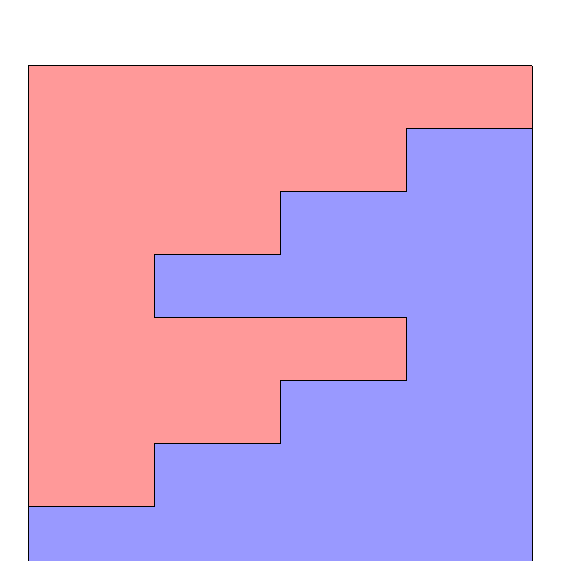
\begin{tikzpicture}[scale=0.8, baseline=(current bounding box.center)]
			
			\draw[black, fill=blue, fill opacity=0.4] (0, 0) -- (8, 0) -- (8, 7) -- (6, 7) -- (6, 6) -- (4, 6) -- (4, 5) -- (2, 5) -- (2, 4) -- (6, 4) -- (6, 3) -- (4, 3) -- (4, 2) -- (2, 2) -- (2, 1) -- (0, 1) -- (0, 0);
			\draw[black, fill=red, fill opacity=0.4] (8, 8) -- (8, 7) -- (6, 7) -- (6, 6) -- (4, 6) -- (4, 5) -- (2, 5) -- (2, 4) -- (6, 4) -- (6, 3) -- (4, 3) -- (4, 2) -- (2, 2) -- (2, 1) -- (0, 1) -- (0, 8) -- (8, 8);
			
		\end{tikzpicture}
		\hfill
		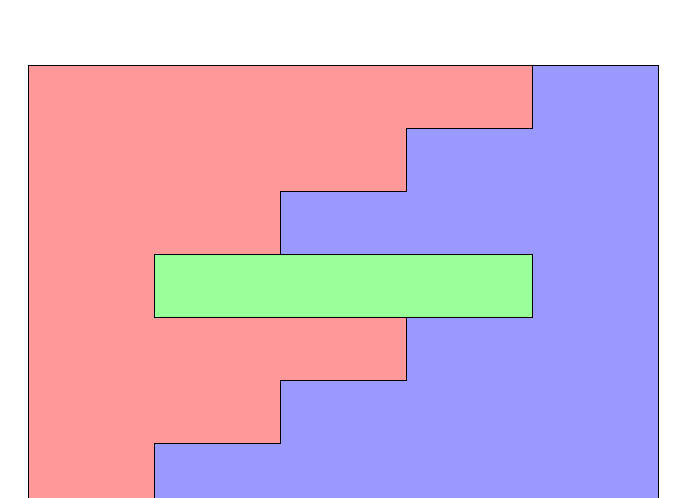
\begin{tikzpicture}[scale=0.8, baseline=(current bounding box.center)]
			
			\draw[black, fill=blue, fill opacity=0.4] (2, 1) -- (10, 1) -- (10, 8) -- (8, 8) -- (8, 7) -- (6, 7) -- (6, 6) -- (4, 6) -- (4, 5) -- (8, 5) -- (8, 4) -- (6, 4) -- (6, 3) -- (4, 3) -- (4, 2) -- (2, 2) -- (2, 1);
			\draw[black, fill=red, fill opacity=0.4] (8, 8) -- (8, 7) -- (6, 7) -- (6, 6) -- (4, 6) -- (4, 5) -- (2, 5) -- (2, 4) -- (6, 4) -- (6, 3) -- (4, 3) -- (4, 2) -- (2, 2) -- (2, 1) -- (0, 1) -- (0, 8) -- (8, 8);
			\draw[black, fill=green, fill opacity=0.4] (2, 4) -- (8, 4) -- (8, 5) -- (2, 5) -- (2, 4);
			
		\end{tikzpicture}
	\end{center}
\end{figure}

\textbf{Extensions and Comments:}

\newpage
\subsection{Semicircle and Quarter Circle Inscribed in Square}

\textbf{Hints:}

\begin{enumerate}
    \item 
\end{enumerate}

\textbf{Solution:}



\textbf{Extensions and Comments:}\newpage
\subsection{Painting a Cube}

During my PGCE at King's College London we were given a simple 10 minute exercise given and then asked to look for extensions. Together with a friend, Amy, we found this extension that the course leader probably was not expecting. Having something to write with will help significantly for this problem, and the initial problem lends itself very well to an explorative approach.

A $4 \times 4 \times 4$ arrangement of cubees form a larger cube. The larger cube is then painted. The original question was to find how many cubees have exactly 1, 2, 3, 4, 5, and 6 faces painted. Find a formula for how many cubees have exactly $k$ painted faces when an $N^m$ hypercube is painted.

\textbf{Hints:}

\begin{enumerate}
    \item 
\end{enumerate}

\textbf{Solution:}



\textbf{Extensions and Comments:}



\newpage
\subsection{Triangles In A Cube}

My dad gave me this problem as a simple problem with a fast answer and said it could be solved within 10 seconds, although I found a way of solving this even faster. I would have expected almost anyone to be able to solve this, although I have been surprised that normal people have pretty poor geometric reasoning abilities. I rate this problem a 1/10 in difficulty.

How many equilateral triangles can be formed by connecting three vertices of a cube?

\textbf{Hints:}

\begin{enumerate}
	\item Connecting any three distinct vertices on the same face will form a right-angled triangle.
	\item Equilateral triangles have rotational symmetry of order 3 - where on a cube do you find such a symmetry?
\end{enumerate}

\textbf{Solution:}

Place three points overlapping at a vertex of the cube. There are three edges connected to this vertex, and we move the points along each of the edges. If all points move along their edge at the same speed then they will form an equilateral triangle by symmetry. Eventually they hit the vertex at the end of the edge, and thus we have found three vertices that form an equilateral triangle. This gives one triangle per vertex, therefore the final answer is 8. We have not shown that these are the only such triangles, although it is not hard to convince yourself by visualising it. The next method proves that these are all the equilateral triangles however.

There are 24 orientation-preserving symmetries of the vertices of a cube, and these form the $O$ group. The vertices of an equilateral triangle have 3 orientation-preserving symmetries and form the $C_3$ group. The quotient set $O/C_3$ has size $\left| \frac{O}{C_3} \right| = \frac{|O|}{|C_3|} = \frac{24}{3} = 8$, and this is the number of triples of vertices with threefold rotational symmetry, in other words, the equilateral triangles.

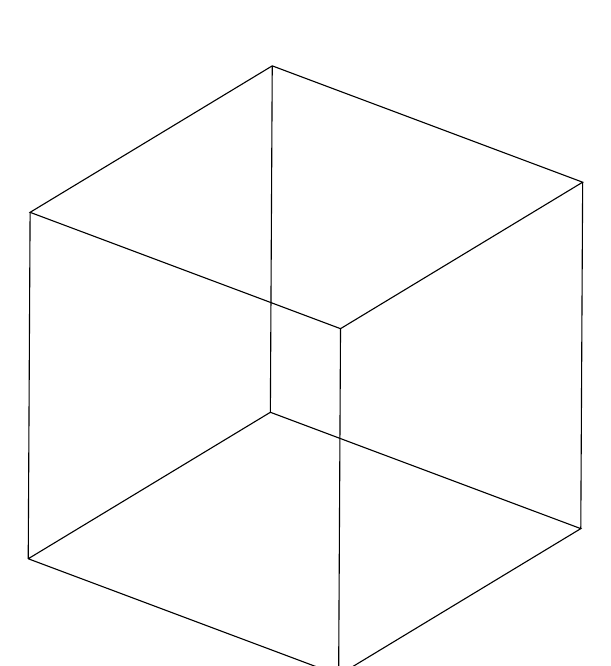
\begin{tikzpicture}[scale=5]
	% Angles used:
	% a = -0.6
	% b = -0.3
	% c =  0.4
	
	% Basis vectors used;
	% 0.47509207, -0.00476773, -0.87992318
	%-0.53942356,  0.78847323, -0.29552021
	% 0.69520483,  0.6150506 ,  0.37202555
	
	\coordinate (V1) at ( 0.00000000,  0.00000000);
	\coordinate (V2) at ( 0.61505060,  0.37202555);
	\coordinate (V3) at ( 0.78847323, -0.29552021);
	\coordinate (V4) at ( 1.40352383,  0.07650535);
	\coordinate (V5) at (-0.00476773, -0.87992318);
	\coordinate (V6) at ( 0.61028287, -0.50789762);
	\coordinate (V7) at ( 0.78370550, -1.17544338);
	\coordinate (V8) at ( 1.39875610, -0.80341783);
	
	\draw (V2) -- (V4) -- (V3) -- (V1) -- (V2);
	\draw (V5) -- (V7) -- (V8) -- (V6) -- (V5);
	\draw (V1) -- (V5);
	\draw (V2) -- (V6);
	\draw (V3) -- (V7);
	\draw (V4) -- (V8);
	
	
\end{tikzpicture}

\textbf{Extensions and Comments:}\newpage
\subsection{Almost Inscribed Triangle In Circle}

I found this from Catriona Agg's collection of geometry problems and it appealed to me as it seemed very minimal. The first solution was found by me and the second simpler solution was found by my dad. I rate this problem a 4 out of 10 in terms of difficulty.

The triangle $ABC$ is equilateral and $|AD| = 9$. Find the area of the circle.

\begin{center}
	\begin{tikzpicture}[scale=3]
		% Defining coordinates
		\coordinate (A) at (0.25, 0.9682458365518544);
\coordinate (B) at (-0.7135254915624212, -0.7006292692220368);
\coordinate (C) at (1.2135254915624212, -0.7006292692220368);
\coordinate (D) at (0.7135254915624212, -0.7006292692220368);
\coordinate (E) at (-0.9635254915624212, -0.26761656732981753);
\coordinate (F) at (0.9635254915624212, 0.26761656732981753);
\coordinate (a) at (0.4817627457812106, 0.13380828366490877);
\coordinate (b) at (0.3658813728906053, 0.5510270601083815);
\coordinate (c) at (0.125, 0.4841229182759272);
\coordinate (d) at (0.5590169943749475, -0.14433756729740643);
		
		\node at (A) [above = 0.1 of A] {$A$};
		\node at (B) [below left = 0.1 of B] {$B$};
		\node at (C) [below right = 0.1 of C] {$C$};
		\node at (D) [below right = 0.1 of D] {$D$};
		\node at (a) [left = 0.2 of a] {$9$};
		
		\draw (0, 0) circle[radius=1];
		\draw (A) -- (B);
		\draw (A) -- (C);
		\draw (A) -- (D);
		\draw (B) -- (C);
	\end{tikzpicture}
\end{center}

\textbf{Hints 1:}

\begin{enumerate}
	\item The triangle $ADC$ contains segment $AC$ which is equal in length to segment $AB$. Use this to construct a congruent triangle.
	\item Prove that the added point of this constructed triangle lies on the circle using the converse of the alternating quadrilateral theorem.
	\item Prove that the triangle formed by $A$, $B$, and the added point is equilateral.
\end{enumerate}

\textbf{Solution 1:}

\begin{figure}[H]
	\begin{center}
		\hfill
		\begin{tikzpicture}[scale=3]
			\coordinate (A) at (0.25, 0.9682458365518544);
\coordinate (B) at (-0.7135254915624212, -0.7006292692220368);
\coordinate (C) at (1.2135254915624212, -0.7006292692220368);
\coordinate (D) at (0.7135254915624212, -0.7006292692220368);
\coordinate (E) at (-0.9635254915624212, -0.26761656732981753);
\coordinate (F) at (0.9635254915624212, 0.26761656732981753);
\coordinate (a) at (0.4817627457812106, 0.13380828366490877);
\coordinate (b) at (0.3658813728906053, 0.5510270601083815);
\coordinate (c) at (0.125, 0.4841229182759272);
\coordinate (d) at (0.5590169943749475, -0.14433756729740643);
	
			\node at (A) [above = 0.1 of A] {$A$};
			\node at (B) [below left = 0.1 of B] {$B$};
			\node at (C) [below right = 0.1 of C] {$C$};
			\node at (D) [below right = 0.1 of D] {$D$};
			\node at (E) [left = 0.1 of E] {$E$};
			\node at (a) [left = 0.2 of a] {$9$};
			
			\draw (0, 0) circle[radius=1];
			
			\draw[fill=blue, fill opacity=0.2] (A) -- (D) -- (C) -- (A);
			\draw[fill=blue, fill opacity=0.2] (A) -- (E) -- (B) -- (A);
			\draw (B) -- (D);
			
			\tkzMarkSegment[pos=0.5, mark=|](A, E);
			\tkzMarkSegment[pos=0.5, mark=|](A, D);
			\tkzMarkSegment[pos=0.5, mark=||](A, B);
			\tkzMarkSegment[pos=0.5, mark=||](A, C);
			
			\pic[draw, angle radius=30, "$60\degree$"] {angle = D--B--A};
			\pic[draw, angle radius=30, "$60\degree$"] {angle = A--C--D};
			\pic[draw, angle radius=30, "$60\degree$"] {angle = A--B--E};
			\pic[draw, angle radius=30, angle eccentricity=1.3, "$\alpha$"] {angle = D--A--C};
			\pic[draw, angle radius=30, angle eccentricity=1.3, "$\alpha$"] {angle = E--A--B};
			\pic[draw, angle radius=30, angle eccentricity=1.3, "$\beta$"] {angle = B--A--D};
			
			\label{fig:AlmostInscribedTriangle_CyclicQuadrilateral}
		\end{tikzpicture}
		\hfill
		\begin{tikzpicture}[scale=3]
			\coordinate (A) at (0.25, 0.9682458365518544);
\coordinate (B) at (-0.7135254915624212, -0.7006292692220368);
\coordinate (C) at (1.2135254915624212, -0.7006292692220368);
\coordinate (D) at (0.7135254915624212, -0.7006292692220368);
\coordinate (E) at (-0.9635254915624212, -0.26761656732981753);
\coordinate (F) at (0.9635254915624212, 0.26761656732981753);
\coordinate (a) at (0.4817627457812106, 0.13380828366490877);
\coordinate (b) at (0.3658813728906053, 0.5510270601083815);
\coordinate (c) at (0.125, 0.4841229182759272);
\coordinate (d) at (0.5590169943749475, -0.14433756729740643);
			
			\node at (A) [above = 0.1 of A] {$A$};
			\node at (B) [below left = 0.1 of B] {$B$};
			\node at (C) [below right = 0.1 of C] {$C$};
			\node at (D) [below right = 0.1 of D] {$D$};
			\node at (E) [left = 0.1 of E] {$E$};
			\node at (a) [left = 0.2 of a] {$9$};
			
			\draw (0, 0) circle[radius=1];
			\draw[fill=red, fill opacity=0.2] (A) -- (E) -- (D) -- (A);
			\draw (A) -- (B);
			\draw (A) -- (C);
			\draw (B) -- (D);
			\draw (B) -- (E);
			\draw (C) -- (D);
			
			\tkzMarkSegment[pos=0.5, mark=|](A, E);
			\tkzMarkSegment[pos=0.5, mark=|](A, D);
			\tkzMarkSegment[pos=0.5, mark=|](E, D);
			
			\pic[draw, angle radius=30, angle eccentricity=1.3, "$60\degree$"] {angle = E--A--D};
			\label{fig:AlmostInscribedTriangle_EquilaterialTriangle}
		\end{tikzpicture}
		\hfill
	\end{center}
	\caption{Solution 1}
\end{figure}

Noting that $|AB| = |AC|$, we construct triangle $EBA$ to be congruent to triangle $DCA$ as shown highlighted in figure~\ref{fig:AlmostInscribedTriangle_CyclicQuadrilateral}. Our aim is to show that the point added to form this triangle, $E$, lies on the circle. Defining $\alpha = \angle BAE$ and $\beta = \angle DAB$, we find $\angle DAE$ by equation~\eqref{eqn:AlmostInscribedTriangleInCircle_AngleDAE}.

\begin{equation}
	\angle DAE = \angle DAB + \angle BAE = \beta + \alpha = \alpha + \beta = \angle CAD + \angle DAB = 60\degree
	\label{eqn:AlmostInscribedTriangleInCircle_AngleDAE}
\end{equation}

By congruence of triangles $EBA$ and $DCA$, $\angle EBA = \angle DCA = 60\degree$, and thus $\angle EBD = 120\degree$. Therefore $\angle EBD$ and $\angle DAE$, opposite angles of quadrilateral $AEBD$, add to $180\degree$. As $\angle AEB$ and $\angle ADC$ are equal by congruence of triangles $EBA$ and $DCA$ and $\angle BDA$ and $\angle ADC$ make the straight line $BDC$, we deduce that opposite angles of quadrilateral $AEBD$ ($\angle AEB$ and $\angle BDA$) add to $180\degree$ as well. Therefore quadrilateral $AEBD$ is a cyclic quadrilateral and thus point $E$ lies on the circle.

By definition $|AD| = |AE|$ which makes triangle $DAE$ isocoles. As shown before, $\angle DAE = 60\degree$, therefore $\angle AED + \angle EDA = 120\degree$. As these angles are equal from triangle $DAE$ being isoceles they must both be $60\degree$, and thus triangle $DAE$ is in fact equilateral. By rotational symmetry the centre of of the triangle must be the centre of the circle. With the simple construction given in figure~\ref{fig:AlmostInscribedTriangle_FindingArea} and basic trigonometry we see that the area of the circle is $27\pi$ as shown in equation~\eqref{eqn:AlmostInscribedTriangleInCircle_ComputingRadiusAndArea}.

\begin{equation}
	r = \frac{4.5}{\sin(60\degree)} = \frac{4.5}{\frac{\sqrt{3}}{2}} = 3\sqrt{3} \implies \text{Area} = \pi r^2 = 27\pi
	\label{eqn:AlmostInscribedTriangleInCircle_ComputingRadiusAndArea}
\end{equation}

\textbf{Hints 2:}

\begin{enumerate}
	\item Find an angle at the centre of the circle.
	\item Draw a kite connecting the circle centre, $A$, $B$, and $D$.
	\item The angle subtended by an arc at the circle centre is double the angle subtended by the same arc at the circle edge.
\end{enumerate}

\textbf{Solution 2:}

Connect the circle centre, $O$, to points $A$ and $D$ to form a kite, as shown in figure~\ref{fig:AlmostInscribedTriangle_Kite} below. As the angle subtended by an arc at the centre is double the angle subtended at the circle edge we get $\angle DOA = 2 \cdot \angle DBA = 120\degree$ and the solution continues identically to solution 1.

\begin{figure}[H]
	\begin{center}
		\hfill
		\begin{tikzpicture}[scale=3]
			\coordinate (A) at (0.25, 0.9682458365518544);
\coordinate (B) at (-0.7135254915624212, -0.7006292692220368);
\coordinate (C) at (1.2135254915624212, -0.7006292692220368);
\coordinate (D) at (0.7135254915624212, -0.7006292692220368);
\coordinate (E) at (-0.9635254915624212, -0.26761656732981753);
\coordinate (F) at (0.9635254915624212, 0.26761656732981753);
\coordinate (a) at (0.4817627457812106, 0.13380828366490877);
\coordinate (b) at (0.3658813728906053, 0.5510270601083815);
\coordinate (c) at (0.125, 0.4841229182759272);
\coordinate (d) at (0.5590169943749475, -0.14433756729740643);
			
			\coordinate (O) at (0, 0);
			
			\node at (A) [above = 0.1 of A] {$A$};
			\node at (B) [below left = 0.1 of B] {$B$};
			\node at (C) [below right = 0.1 of C] {$C$};
			\node at (D) [below right = 0.1 of D] {$D$};
			\node at (O) [left = 0.15 of O] {$O$};
			\node at (d) [right = 0.15 of d] {$9$};
			
			\draw (O) circle[radius=1];
			\draw (A) -- (C);
			\draw (C) -- (D);
			\draw (A) -- (D);
			\draw[fill=blue, fill opacity=0.2] (A) -- (B) -- (D) -- (O) -- (A);
			
			\pic[draw, angle radius=30, "\hspace{2mm}$60\degree$"] {angle = D--B--A};
			\pic[draw, angle radius=30, "$120\degree$"] {angle = D--O--A};
			
			\label{fig:AlmostInscribedTriangle_Kite}
		\end{tikzpicture}
		\hfill
		\begin{tikzpicture}[scale=3]
			\coordinate (A) at (0.25, 0.9682458365518544);
\coordinate (B) at (-0.7135254915624212, -0.7006292692220368);
\coordinate (C) at (1.2135254915624212, -0.7006292692220368);
\coordinate (D) at (0.7135254915624212, -0.7006292692220368);
\coordinate (E) at (-0.9635254915624212, -0.26761656732981753);
\coordinate (F) at (0.9635254915624212, 0.26761656732981753);
\coordinate (a) at (0.4817627457812106, 0.13380828366490877);
\coordinate (b) at (0.3658813728906053, 0.5510270601083815);
\coordinate (c) at (0.125, 0.4841229182759272);
\coordinate (d) at (0.5590169943749475, -0.14433756729740643);
			
			\coordinate (O) at (0, 0);
			
			\node at (A) [above = 0.1 of A] {$A$};
			\node at (D) [below right = 0.1 of D] {$D$};
			\node at (O) [left = 0.15 of O] {$O$};
			\node at (F) [right = 0.15 of F] {$F$};
			\node at (b) [right = 0.1 of b] {$4.5$};
			\node at (c) [left = 0.1 of c] {$r$};
			
			\draw (O) circle[radius=1];
			\draw (A) -- (D);
			\draw (O) -- (A);
			\draw (O) -- (D);
			\draw (O) -- (F);
			
			\pic[draw, angle radius=30, "\hspace{2mm}$60\degree$"] {angle = F--O--A};
			\pic[draw, angle radius=10] {right angle = A--a--O};
			
			\label{fig:AlmostInscribedTriangle_FindingArea}
		\end{tikzpicture}
		\hfill
	\end{center}
	\caption{Solution 2 and the common method for finding the circle area}
\end{figure}

\textbf{Extensions and Comments:}

I tried solving this while on the train and was not bothered to get my whiteboard out. I managed to find and prove the cyclic quadrilateral, but did not spot the isocoles triangle which would have made the problem trivial.
\newpage
\stopcontents\newpage
\section{Physics}

\thispagestyle{subcontents}

\vspace{-5mm}
\startcontents
\printcontents{}{1}{\section*{\contentsname}}
\clearpage

\subsection{The Ball and the Boat Problem}

This is a classic problem, but I first did a proper analysis of it when I was looking for Oxbridge mock interview questions and my friend, Dami from WSP, suggested it. This requires only very basic understanding of physics and does not need any particular tricks or special insights to solve, but is nevertheless quite pleasing. I rate this problem a 2 out of 10 in terms of difficulty.

Suppose there is a small boat in a pool with a person and a ball onboard. The person throws the ball overboard. What happens to the water level in the following cases?

\begin{enumerate}
    \item The ball sinks to the bottom.
    \item The ball floats on the surface.
    \item The ball floats but it is then tied to the bottom of the pool.
    \item The ball floats but the person in the boat forces it underwater so it is fully submerged.
\end{enumerate}

\textbf{Hints:}

\begin{enumerate}
    \item Remember Archimedes' principle - the buoyant force acting on an object is equal to the weight of fluid it displaces, and acts in the upwards direction.
    \item Consider extreme cases - a very dense ball and a ball with very low density.
    \item Identify the different systems and the forces acting on them.
\end{enumerate}

\textbf{Solution:}

The key to this problem is understanding difference between buoyant forces caused by the mass of the ball and the volume of the ball. When the ball is in the boat, the buoyant force is due to the weight of the ball and is independent of the volume. When the ball is in the water, the buoyant force is due to the volume of the ball and is independent of the weight. The forces in the original situation are shown in figure~\ref{fig:TheBallAndTheBoat_Setup}, and the four cases are shown in figure~\ref{fig:TheBallAndTheBoat}.

When the ball is in the boat, the additional weight pushes the boat deeper into the water, meaning a greater volume of the boat is under the water line. This means a greater volume of water is displaced, and thus a greater weight of water is displaced, and therefore a larger buoyant force. This force is a function only of the weight of the ball as changing the volume of the ball only displaces air inside the boat. When the ball is fully submerged, the volume of water displaced is equal to the volume of the ball and therefore the weight of the ball is irrelevant. If the ball is floating, then by Archimedes' principle the weight of the water displaced by the volume of the ball is equal to the weight of the ball.

This understanding can be used to construct a force balance. When the ball is in the boat, the boat and the ball are treated together as a single system. The two forces are the weight of the ball and the boat combined acting downwards, and an equal and opposite buoyant force acting upwards. When the ball is fully submerged, the ball and the boat need to be treated as separate systems. As before, the boat has two forces acting on it, the weight of the boat and the equal and opposite buoyant force. The case for the ball is different however. The ball has a weight acting downwards, but now there are two forces acting upwards. The buoyant force is equal to the weight of water displaced by the ball and there is also a reaction force from the bottom of the pool stopping the ball falling through the floor.

In both cases, the systems are in equilibrium and the total downwards forces are equal, meaning the upwards forces must be equal in both cases as well. As there is a contact force when the ball is submerged, the total buoyant force must be less than when the ball is in the boat. The buoyant force is equal to the weight of the water displaced, and as the water is of constant density, this is proportional to the volume of water displaced. This means less water is displaced when the ball is submerged compared to being in the boat, and thus the water level is lower. We could also see this by noting the weight of the ball must be greater than the weight of the water it displaces because it is denser than water.

Similar reasoning can be applied in the other parts of the question. If the ball floats on the surface or has a density equal to that of water there is no contact force. The total system weight is equal to the total system buoyant force in both cases, meaning the water level stays the same. If the ball has a density less than water but is forced under the surface anyway, the buoyant force is more than the weight. Instead of a contact force acting upwards, a tension in the rope acts downwards to maintain equilibrium. The greater total buoyant force means more water is displaced, giving a higher water level.

The final part is almost identical to the second part. The total buoyant force is equal to the total weight as there are no other forces acting on the system and it is in equilibrium. As before this leads to the water lever staying the same. Understanding the individual forces on the ball and boat is still interesting however. The buoyant force on the ball is split into two parts, one equal to the weight of the ball, and the remaining buoyancy is additional buoyancy. As the weight of the boat is smaller than the boat and the ball combined, the boat will float higher in the water due to a smaller volume needing to be displaced. This loss in buoyancy is exactly equal to the additional buoyancy from the ball. Compared to the second part of the question, the boat sits higher in the water and the ball sits lower, with the total water displaced remaining exactly equal.

\textbf{Extensions and Comments:}

This is a problem where thinking of extreme cases helps elucidate the principles. Consider a very tiny ball of constant size and large mass. The difference in water level when the ball is in the water or completely removed from the system is negligible due to the small size of the ball. Increasing the weight makes no difference at all. If the ball was put into the boat however, the boat would sit much lower in the water. Increasing the weight of the ball would cause it to sit even lower, and clearly the volume of water displaced increases. A very light ball with a large varying volume demonstrates part three nicely. This makes very little difference to how deep the boat sits in the water, and is independent of the volume. When increasing the volume when it is submerged, the volume of water displaced increases, and the water level clearly increases.

\begin{figure}[H]
    \centering
    \begin{subfigure}{0.49\textwidth}
        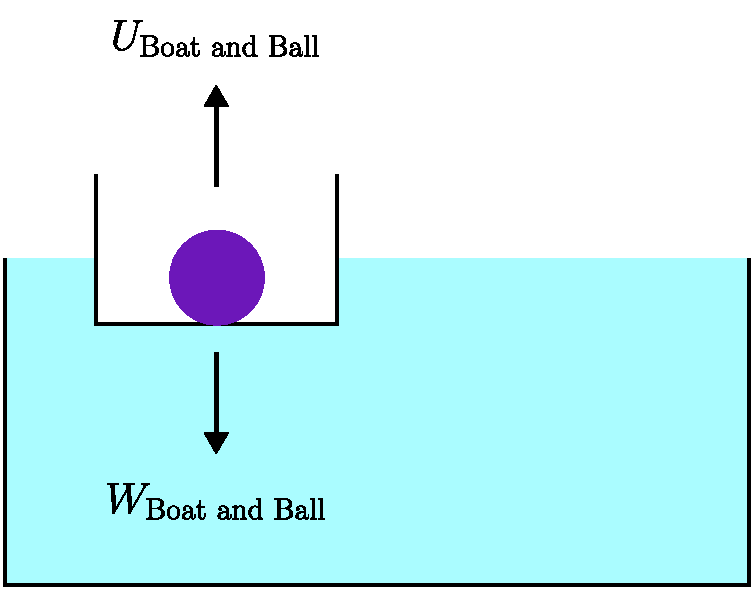
\includegraphics[width=\textwidth]{5 - Physics/TheBallAndTheBoat_Setup.pdf}
    \end{subfigure}
    \caption{The forces acting on the original system}
    \label{fig:TheBallAndTheBoat_Setup}
\end{figure}

\begin{figure}[H]
    \centering
    \begin{subfigure}{0.49\textwidth}
        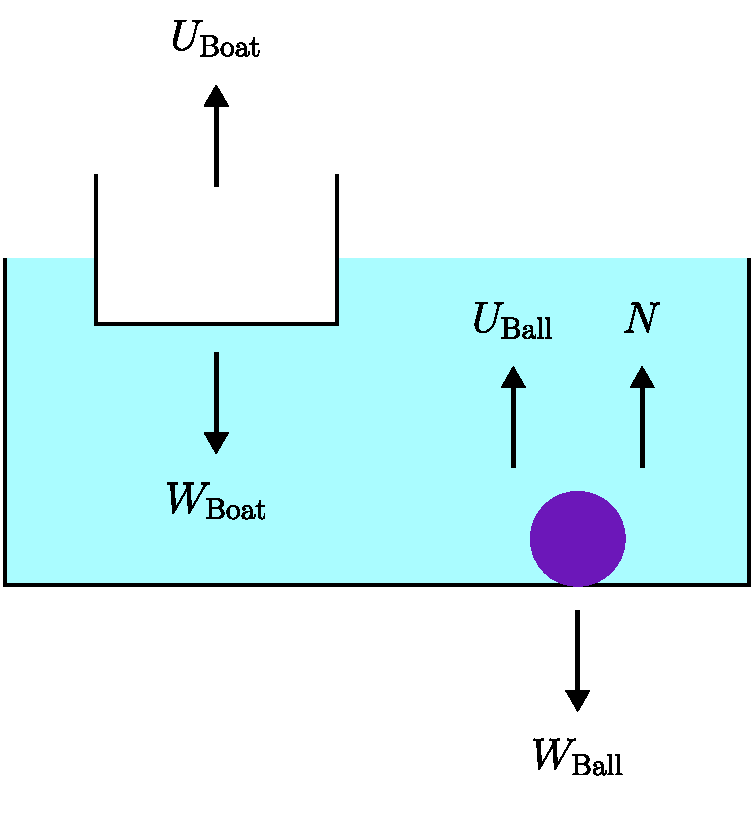
\includegraphics[width=\textwidth]{5 - Physics/TheBallAndTheBoat_Case1.pdf}
        \caption{Part 1}
        \label{fig:TheBallAndTheBoat_Case1}
    \end{subfigure}
    \hfill
    \begin{subfigure}{0.49\textwidth}
        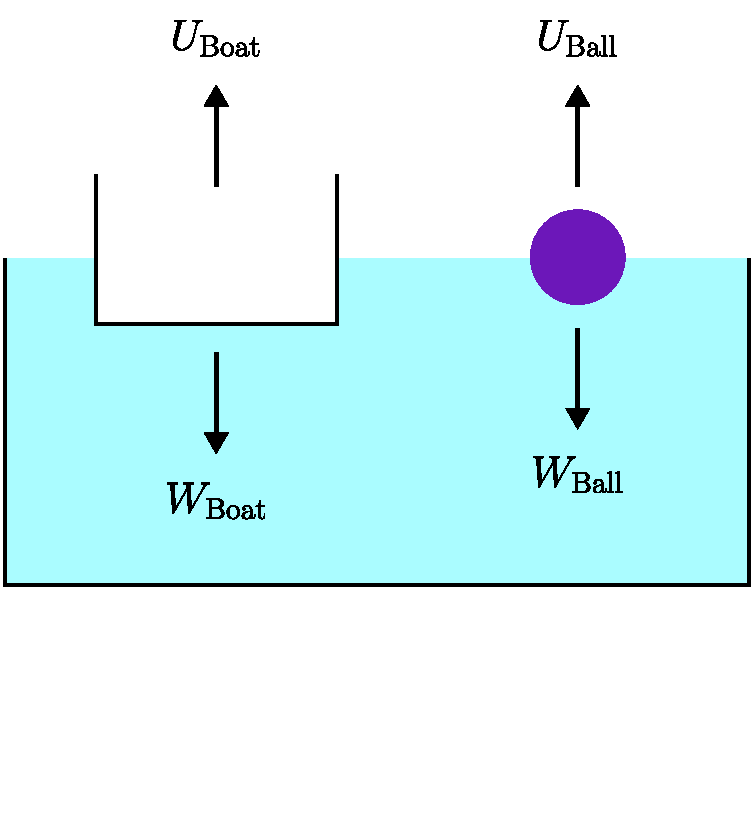
\includegraphics[width=\textwidth]{5 - Physics/TheBallAndTheBoat_Case2.pdf}
        \caption{Part 2}
        \label{fig:TheBallAndTheBoat_Case2}
    \end{subfigure}  \\
    \vspace{10mm}
    \begin{subfigure}{0.49\textwidth}
        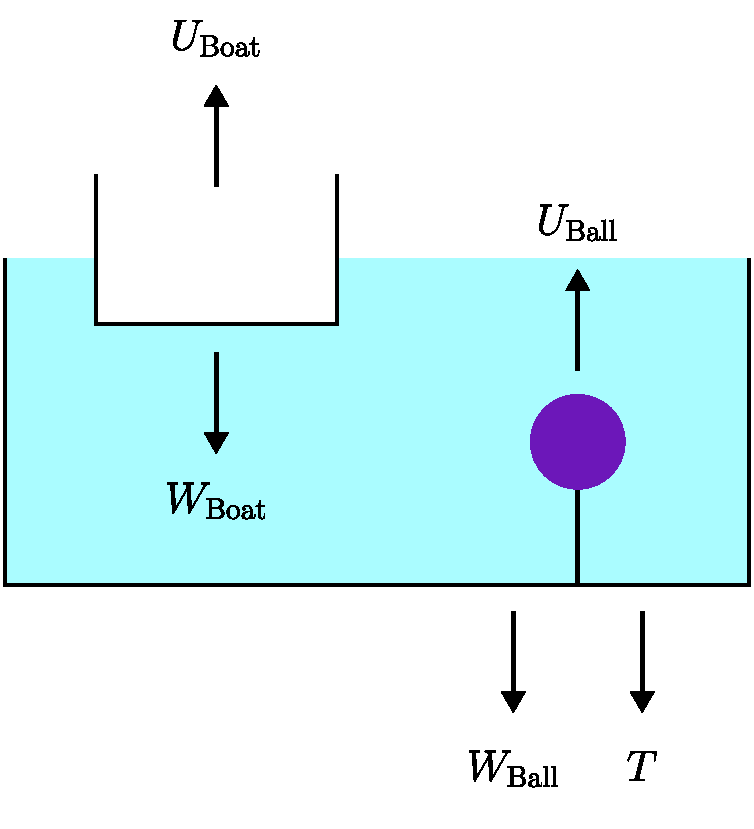
\includegraphics[width=\textwidth]{5 - Physics/TheBallAndTheBoat_Case3.pdf}
        \caption{Part 3}
        \label{fig:TheBallAndTheBoat_Case3}
    \end{subfigure}
    \hfill
    \begin{subfigure}{0.49\textwidth}
        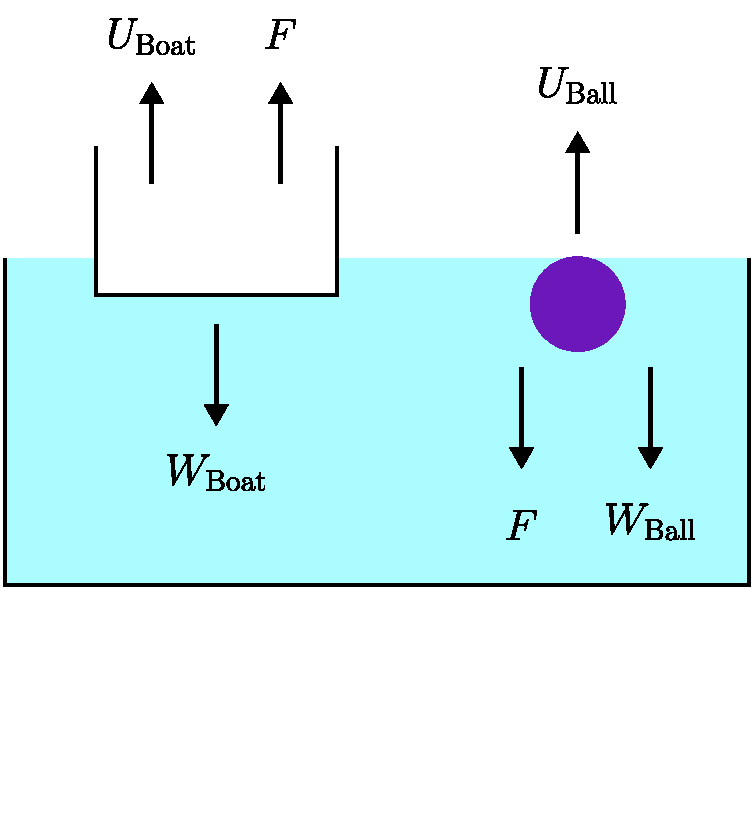
\includegraphics[width=\textwidth]{5 - Physics/TheBallAndTheBoat_Case4.pdf}
        \caption{Part 4}
        \label{fig:TheBallAndTheBoat_Case4}
    \end{subfigure}
    \caption{The forces acting on the ball and the boat in each of the four parts}
    \label{fig:TheBallAndTheBoat}
\end{figure}

\stopcontents\newpage

\newpage

% Add Josepheus problem
% Add spherical polar basis problem
% Add umbrella problem
% Add semicircle and quarter circle in square problem

\fancyhf{}
\fancyhead[L]{References}
\fancyhead[R]{}
\fancyfoot[C]{\thepage}

\addcontentsline{toc}{section}{References}
\bibliographystyle{unsrtHenry.bst}
\bibliography{bibliography.bib}

\end{document}